\documentclass{beamer}
\usetheme{Boadilla}
\usecolortheme{crane}
\usefonttheme[stillsansseriflarge, stillsansserifsmall]{serif}
%\usefonttheme[stillsansseriflarge, stillsansserifsmall]{structurebold}
%\usefonttheme[onlymath]{serif}
\useinnertheme{default}

\usepackage{fontspec}
\usepackage{kpfonts}
%\setmainfont[Numbers=OldStyle]{Tex Gyre Pagella}
\setsansfont[BoldFont=Lovelo-LineBold]{Lovelo-LineBold}

\usepackage[frenchb]{babel}


%proper math and math symbols
%\usepackage{amsmath}
\usepackage{amssymb}

\usepackage{siunitx}
\usepackage{booktabs}
\usepackage{multirow}

% Allow the usage of graphics (.jpg, .png, etc.) in the document
\usepackage{graphicx}
\usepackage{tikz}
\usetikzlibrary{arrows,shapes,backgrounds, positioning, intersections, decorations.markings, mindmap, shapes.geometric, matrix, shapes.callouts,patterns}

\usepackage{pgfplots}
%\usepgfplotslibrary{units}
\usepgfplotslibrary{groupplots}
\usepgfplotslibrary{external}
\tikzset{external/system call={lualatex \tikzexternalcheckshellescape -halt-on-error -interaction=batchmode -jobname "\image" "\texsource"}}

%\tikzexternalize

%bibliography
\usepackage{natbib}
%\usepackage{bibentry}
\def\newblock{\hskip .11em plus .33em minus .07em}

\institute{ENS Lyon}
\title{Réunion hebdomadaire}

\author[M. Leocmach]{Mathieu Leocmach}
\date{26 June 2013}

\begin{document}
\tikzset{every mark/.append style={scale=0.8}}
\pgfplotsset{every axis/.append style={small}}
\tikzset{external/force remake=false}

\AtBeginSection[]{
	\addtocounter{framenumber}{-1}
	\begin{frame}[plain]
		\tableofcontents[currentsection, hideothersubsections]
	\end{frame}
}

\begin{frame}[plain]
	\titlepage
\end{frame}

\begin{frame}{Relier deux phénomènes}
\begin{columns}
\column{0.5\textwidth}
Fractures sous contrainte

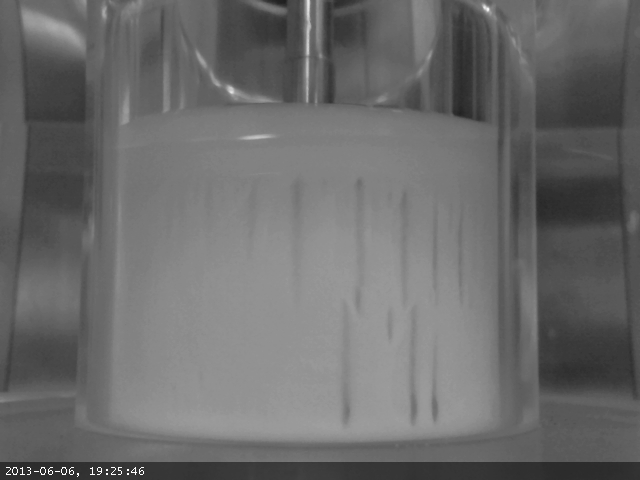
\includegraphics[width=\columnwidth]{gap1mm_Y191_SSC300.jpg}

\column{0.5\textwidth}
Motif sans attache

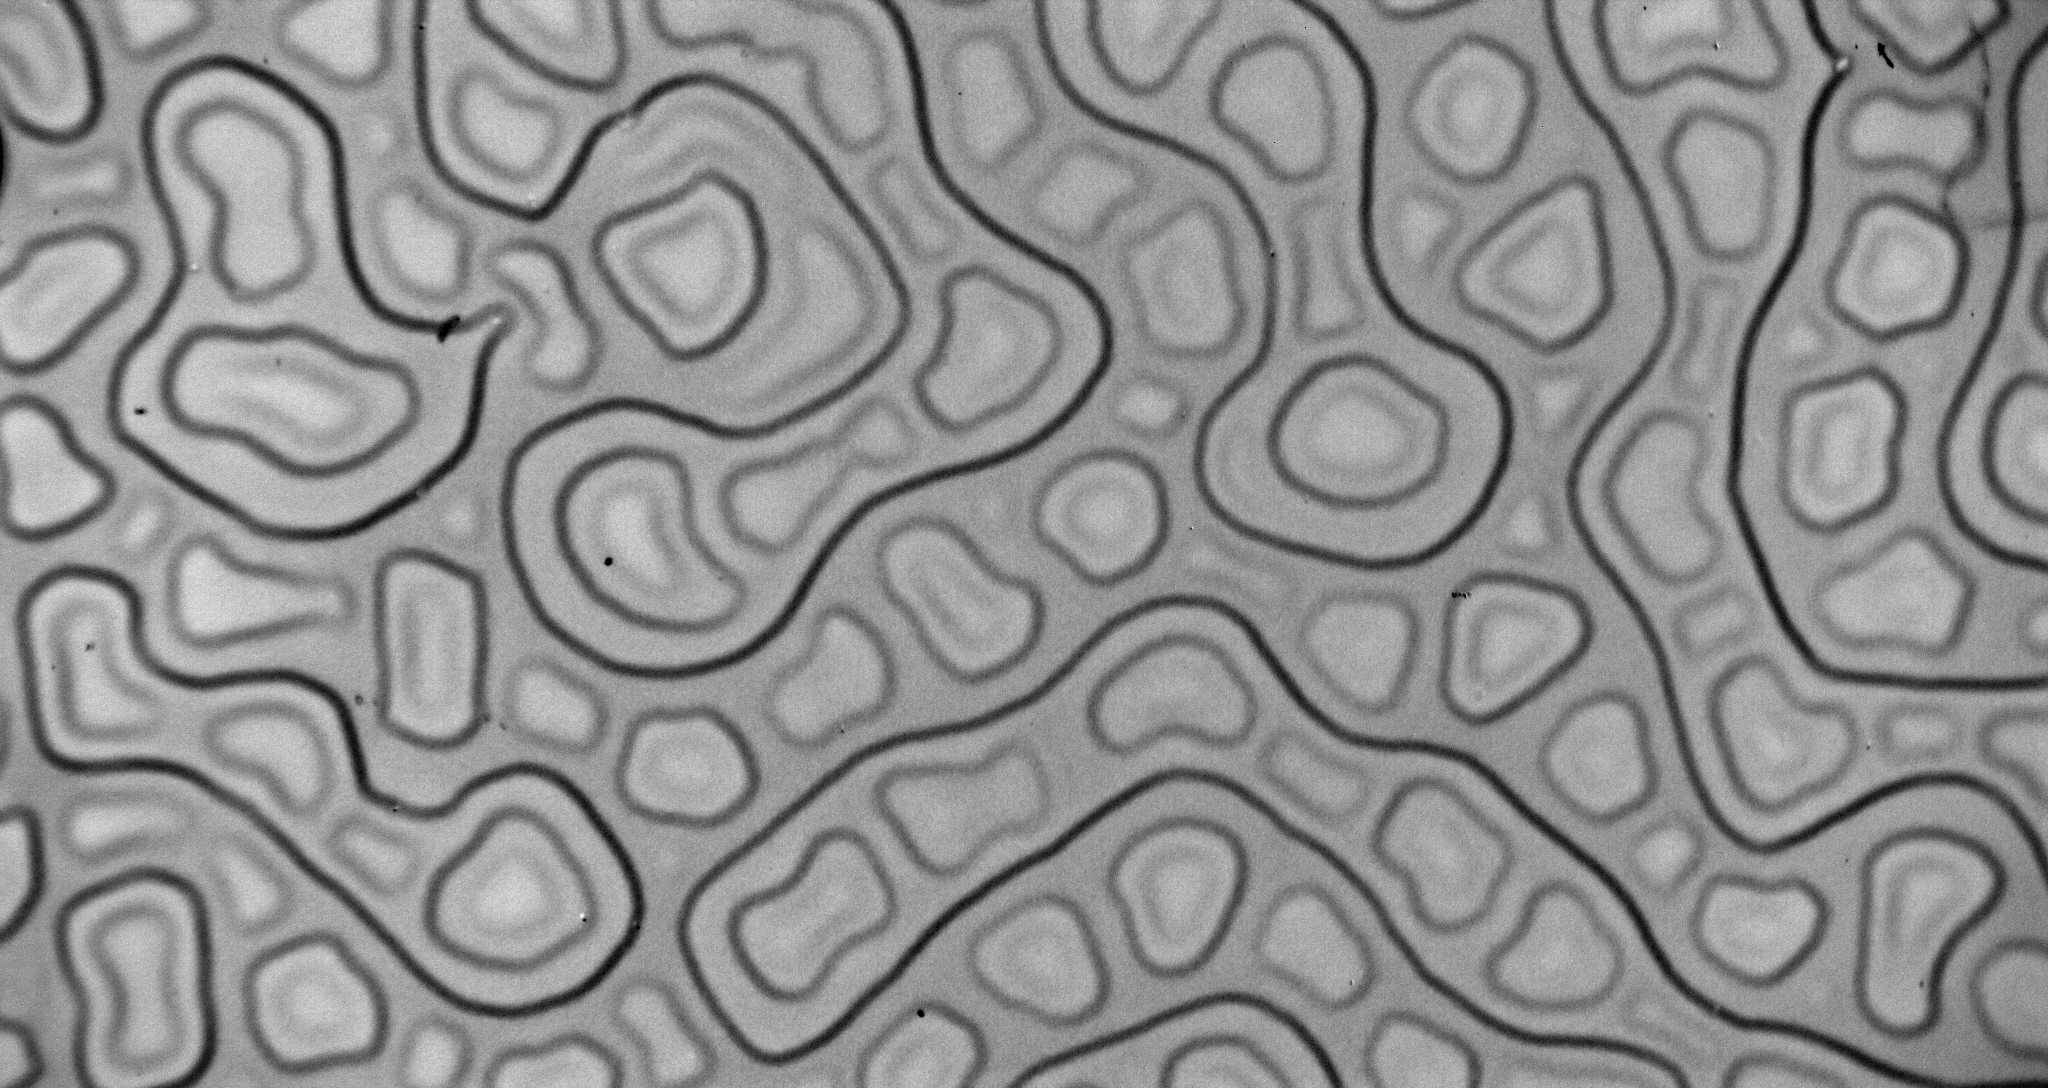
\includegraphics[width=\columnwidth]{pattern_100um.png}

\end{columns}
\end{frame}

\begin{frame}{Fractures sous contrainte: Fluage}
\begin{columns}
\column{0.6\textwidth}
\begin{tikzpicture}
\begin{loglogaxis}[%
	xlabel={$t\,(s)$},
	ylabel={Taux de déformation $(s^{-1})$},
	]
	\addplot[no marks] file {Y34_strain_rate_log.txt};
	\draw[<->] (axis cs:1e-1,1) -- (axis cs:1.3e3,5e-4) node[midway,above,rotate=-21] {régime d'Andrade};
	\node at (axis cs:1.3e3,1e-4) (det){};
	\node at (axis cs:2.3e3,1e4) (touch){};
\end{loglogaxis}
\draw[<-, red, ultra thick] (det) -- ++(0,-4em) node[left] {Apparition des fractures};
\draw[<-, red, ultra thick] (touch) -- ++(0,3em) node[left] {Les fractures se rejoignent};
\end{tikzpicture}
\column{0.4\textwidth}
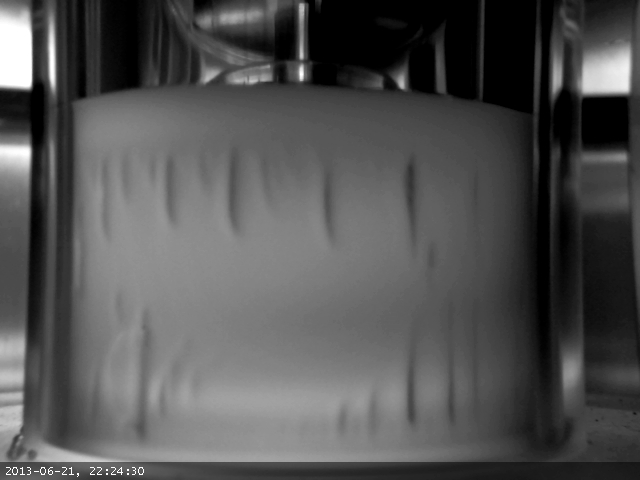
\includegraphics[width=\columnwidth, trim=0 0 0 1cm,clip=true]{Y210_SSC300_avant_div.jpg}

\begin{tikzpicture}[inner sep=0]
\node[anchor=north east]{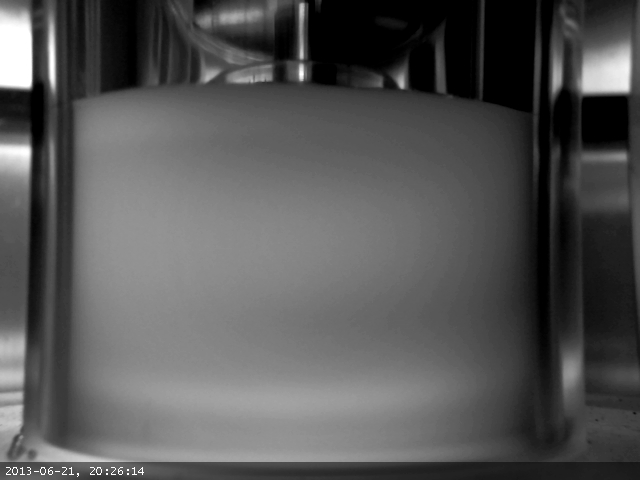
\includegraphics[width=\columnwidth, trim=0 0 0 1cm,clip=true]{Y210_SSC300_premiere_frac.jpg}};
\node[anchor=north east]{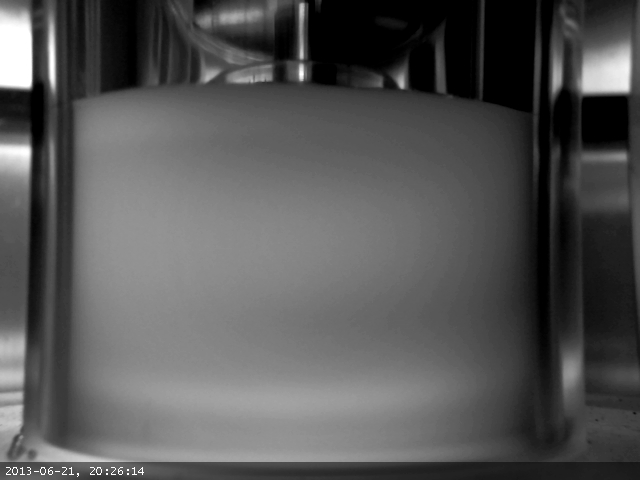
\includegraphics[width=0.5\columnwidth,% trim=1cm 6mm 15cm 12cm,clip=true]{Y210_SSC300_premiere_frac.jpg}};
]{detail_premiere_frac.jpg}};
\draw[red,radius=0.05\columnwidth] (-0.775\columnwidth,-0.625\columnwidth) circle;
\draw[red,radius=0.06\columnwidth] (-0.29\columnwidth,-0.25\columnwidth) circle;
\end{tikzpicture}
\end{columns}
\end{frame}

\begin{frame}{Fractures sous contrainte: Décollement}
\begin{tikzpicture}
\begin{axis}[%
	scale only axis,
	xmin=0,xmax=2322,
	ymin=0, ymax=1100,
	ylabel={$r_\text{gap}\,(\mu m)$},
	axis on top,
	xtick={0,500,1000,1500,2000},
	]
	\addplot graphics[
		xmin=0,xmax=2322,
		ymin=0,ymax=1100,
		]{spatioY34};
\end{axis}
\begin{semilogyaxis}[%
	scale only axis,
	xmin=0,xmax=2322,
	%ymin=0, ymax=1100,
	axis y line*=right,
	axis x line=none,
	ylabel={Taux de déformation $(s^{-1})$},
	ylabel near ticks,
	]
	\addplot[no marks] file {Y34_strain_rate_log.txt};
	\node at (axis cs:1.3e3,2e-4) (a) {};
	\draw[green!50!black, dashed] (axis cs:2.18e3,1e-4) -- (axis cs:2.18e3,1e4) node (b) {};
\end{semilogyaxis}
\draw[<-, green!50!black, ultra thick] (a) -- ++(0,-3.5em) node[left] {Première fracture au bord};
\draw[<-, green!50!black, ultra thick] (b) -- ++(0,2em) node[left] {Une fracture atteint le niveau du transducteur};
\end{tikzpicture}
\end{frame}

\begin{frame}{Fractures sous contrainte: exp ou pow ?}
\begin{columns}
\column{0.6\textwidth}
\begin{tikzpicture}
\begin{axis}[%
	name=phasediag,
	xlabel near ticks,
	ylabel near ticks,
	xmin=0,xmax=5,xlabel={\% caseinate},
	ymin=0,ymax=5,ylabel={\% GDL},
	legend style={legend pos=north west,},
	]
\addplot[mark=triangle*, green!50!black, only marks] coordinates {(4,3) (4,2) (4,1)};
\addplot[mark=square*, red, only marks] coordinates {(1,1)};
\addplot[mark=diamond*, orange, only marks] coordinates {(4,4)};\legend{puissance, exponentielle, coexistence};
\addplot[no marks, dotted, black] coordinates {(0,0) (5,5) (10,5) (0,0) (8,2)};
\node at (axis cs:4.5,4.5) {1h};
\node at (axis cs:4.5,1.125) {8h};
\end{axis}
\draw[->] ($(phasediag.north east)+(1em,0)$) -- ($(phasediag.south east)+(1em,0)$) node[midway,right] {$G^{\prime}\nearrow$};
\draw[->] ($(phasediag.north west)+(0,1em)$) -- ($(phasediag.north east)+(0,1em)$) node[midway,above] {$G^{\prime}\nearrow$};
\end{tikzpicture}
\column{0.4\textwidth}
$\tau_\text{casse}(\sigma)$
\begin{itemize}
\item \textcolor{green!50!black}{fractures $\Leftrightarrow$ loi de puissance}
\item \textcolor{red}{pas de fracture $\Leftrightarrow$ exponentielle}
\end{itemize}
Pour le 4\% 4\%, fractures et loi de puissance à bas stress, pas de fractures et exponentielle à haut stress.
\end{columns}
\end{frame}

\begin{frame}{Fractures sous contrainte: exp ou pow ?}
\begin{tikzpicture}
\begin{groupplot}[%
	group style={
		group size=2 by 1, 
		y descriptions at=edge left,
		horizontal sep=1em,
		},
	ymode=log,
	ylabel={$\tau_\text{casse}$ (s)},ylabel near ticks,
	xlabel={$\sigma$ (Pa)},
	]
	\nextgroupplot[
		xmode=normal,
		xmin=0,
		legend style={legend pos=north east,},
		]
	\draw (axis cs:200,1e3) -- (axis cs:700,5);
	\draw (axis cs:2,1.7e4) -- (axis cs:40,7.85e-1);
	\addplot+[only marks,mark=triangle, green!50!black] table[x index=0, y index=1]{cas4_GDL1_t_cassure_sigma.txt};
	\addplot+[only marks,mark=diamond, orange] table[x index=0, y index=2]{cas4_GDL4_t_cassure_sigma.txt};
	\addplot+[only marks,mark=square, red] table[x index=0, y index=2]{cas1_GDL1_t_cassure_sigma.txt};
	\legend{4\% 1\%, 4\% 4\%, 1\% 1\%};
	%
	
	\nextgroupplot[xmode=log]
	\draw (axis cs:150,5e5) -- (axis cs:1000,25);
	\draw (axis cs:30,1e5) -- (axis cs:200,2e3);
	\addplot+[only marks,mark=triangle, green!50!black] table[x index=0, y index=1]{cas4_GDL1_t_cassure_sigma.txt};
	\addplot+[only marks,mark=diamond, orange] table[x index=0, y index=2]{cas4_GDL4_t_cassure_sigma.txt};
	\addplot+[only marks,mark=square, red] table[x index=0, y index=2]{cas1_GDL1_t_cassure_sigma.txt};
\end{groupplot}
\end{tikzpicture}
Note: Dans le 4\% 4\% le préfacteur dépend du gap.
\end{frame}

\begin{frame}{Fractures sous contrainte: exp ou pow ?}
On voit la transition dans la colonne 4\% de caséine.
\begin{tikzpicture}
\begin{groupplot}[%
	group style={
		group size=2 by 1, 
		y descriptions at=edge left,
		horizontal sep=1em,
		},
	ymode=log,
	ylabel={$\tau_\text{casse}$ (s)},ylabel near ticks,
	xlabel={$\sigma$ (Pa)},
	]
	\nextgroupplot[
		xmode=normal,
		xmin=0,
		legend style={legend pos=north east,},
		]
	%\draw (axis cs:200,1e3) -- (axis cs:700,5);
	%\draw (axis cs:2,1.7e4) -- (axis cs:40,7.85e-1);
	\addplot+[only marks,mark=triangle, green!50!black] table[x index=0, y index=1]{cas4_GDL1_t_cassure_sigma.txt};
	\addplot+[only marks,mark=*, blue,mark options={fill=blue}] table[x index=1, y index=2]{cassure_cas4_GDL2.csv};
	\addplot+[only marks,mark=pentagon*, purple,mark options={fill=purple}] table[x index=1, y index=2]{cassure_cas4_GDL3.csv};
	\addplot+[only marks,mark=diamond, orange] table[x index=0, y index=2]{cas4_GDL4_t_cassure_sigma.txt};
	\legend{4\% 1\%, 4\% 2\%, 4\% 2\%, 4\% 1\%};
	%
	
	\nextgroupplot[xmode=log]
	\draw (axis cs:150,5e5) -- (axis cs:1000,25);
	\draw (axis cs:30,1e5) -- (axis cs:200,2e3);
	\draw (axis cs:100,131182) -- (axis cs:200,16251);
	\draw (axis cs:100,2e4) -- (axis cs:300,1.7e3);
	\addplot+[only marks,mark=triangle, green!50!black] table[x index=0, y index=1]{cas4_GDL1_t_cassure_sigma.txt};
	\addplot+[only marks,mark=*, blue,mark options={fill=blue}] table[x index=1, y index=2]{cassure_cas4_GDL2.csv};
	\addplot+[only marks,mark=pentagon*, purple,mark options={fill=purple}] table[x index=1, y index=2]{cassure_cas4_GDL3.csv};
	\addplot+[only marks,mark=diamond, orange] table[x index=0, y index=2]{cas4_GDL4_t_cassure_sigma.txt};
\end{groupplot}
\end{tikzpicture}
\end{frame}

\begin{frame}{Motifs: Ingrédients}
\begin{center}
\begin{tikzpicture}
\fill[pattern=north east lines,pattern color=blue] (0,0) rectangle (12,0.5) node[midway,fill=white,inner sep=1pt] {verre};
\fill[pattern=north east lines,pattern color=blue] (0,-1) rectangle (12,-1.5) node[midway,fill=white,inner sep=1pt] {verre};
\draw[blue,line width=2pt,green!80!black] (0,-1) -- (12,-1) (0,-1pt) -- (12,-1pt) node[below,pos=0.30] {brosse acrylamide ($10\sim 100$ nm)};
\fill[gray] (0,0) rectangle (0.5,-1) (12,0) rectangle (11.5,-1) node[pos=0.75, left] {spacer};
\draw[<->] (9,-2pt) -- (9,-1) node[midway,left] {$e\sim 100\,\mu m$};
\draw[<->] (0.5,0.75) -- (11.5,0.75) node[midway,above] {$L\sim 2.5cm$};
\end{tikzpicture}
\end{center}

\begin{itemize}
\item Pas d'accroche sur les plus grandes surfaces grâce aux brosses.
\item Accroche sur les extrémités (spacers solides, pas d'interface libre)
\item Contraintes auto-générées par la séparation de phase/gélification
\end{itemize}
\end{frame}

\begin{frame}{Motifs: Formation}
%\movie{\includegraphics[width=.9\textwidth]{une_image.jpg}}{videos/une_video.avi}
\end{frame}

\begin{frame}{Motifs: Structure}
\begin{columns}
\column{0.6\textwidth}
\begin{tabular}{ccc}
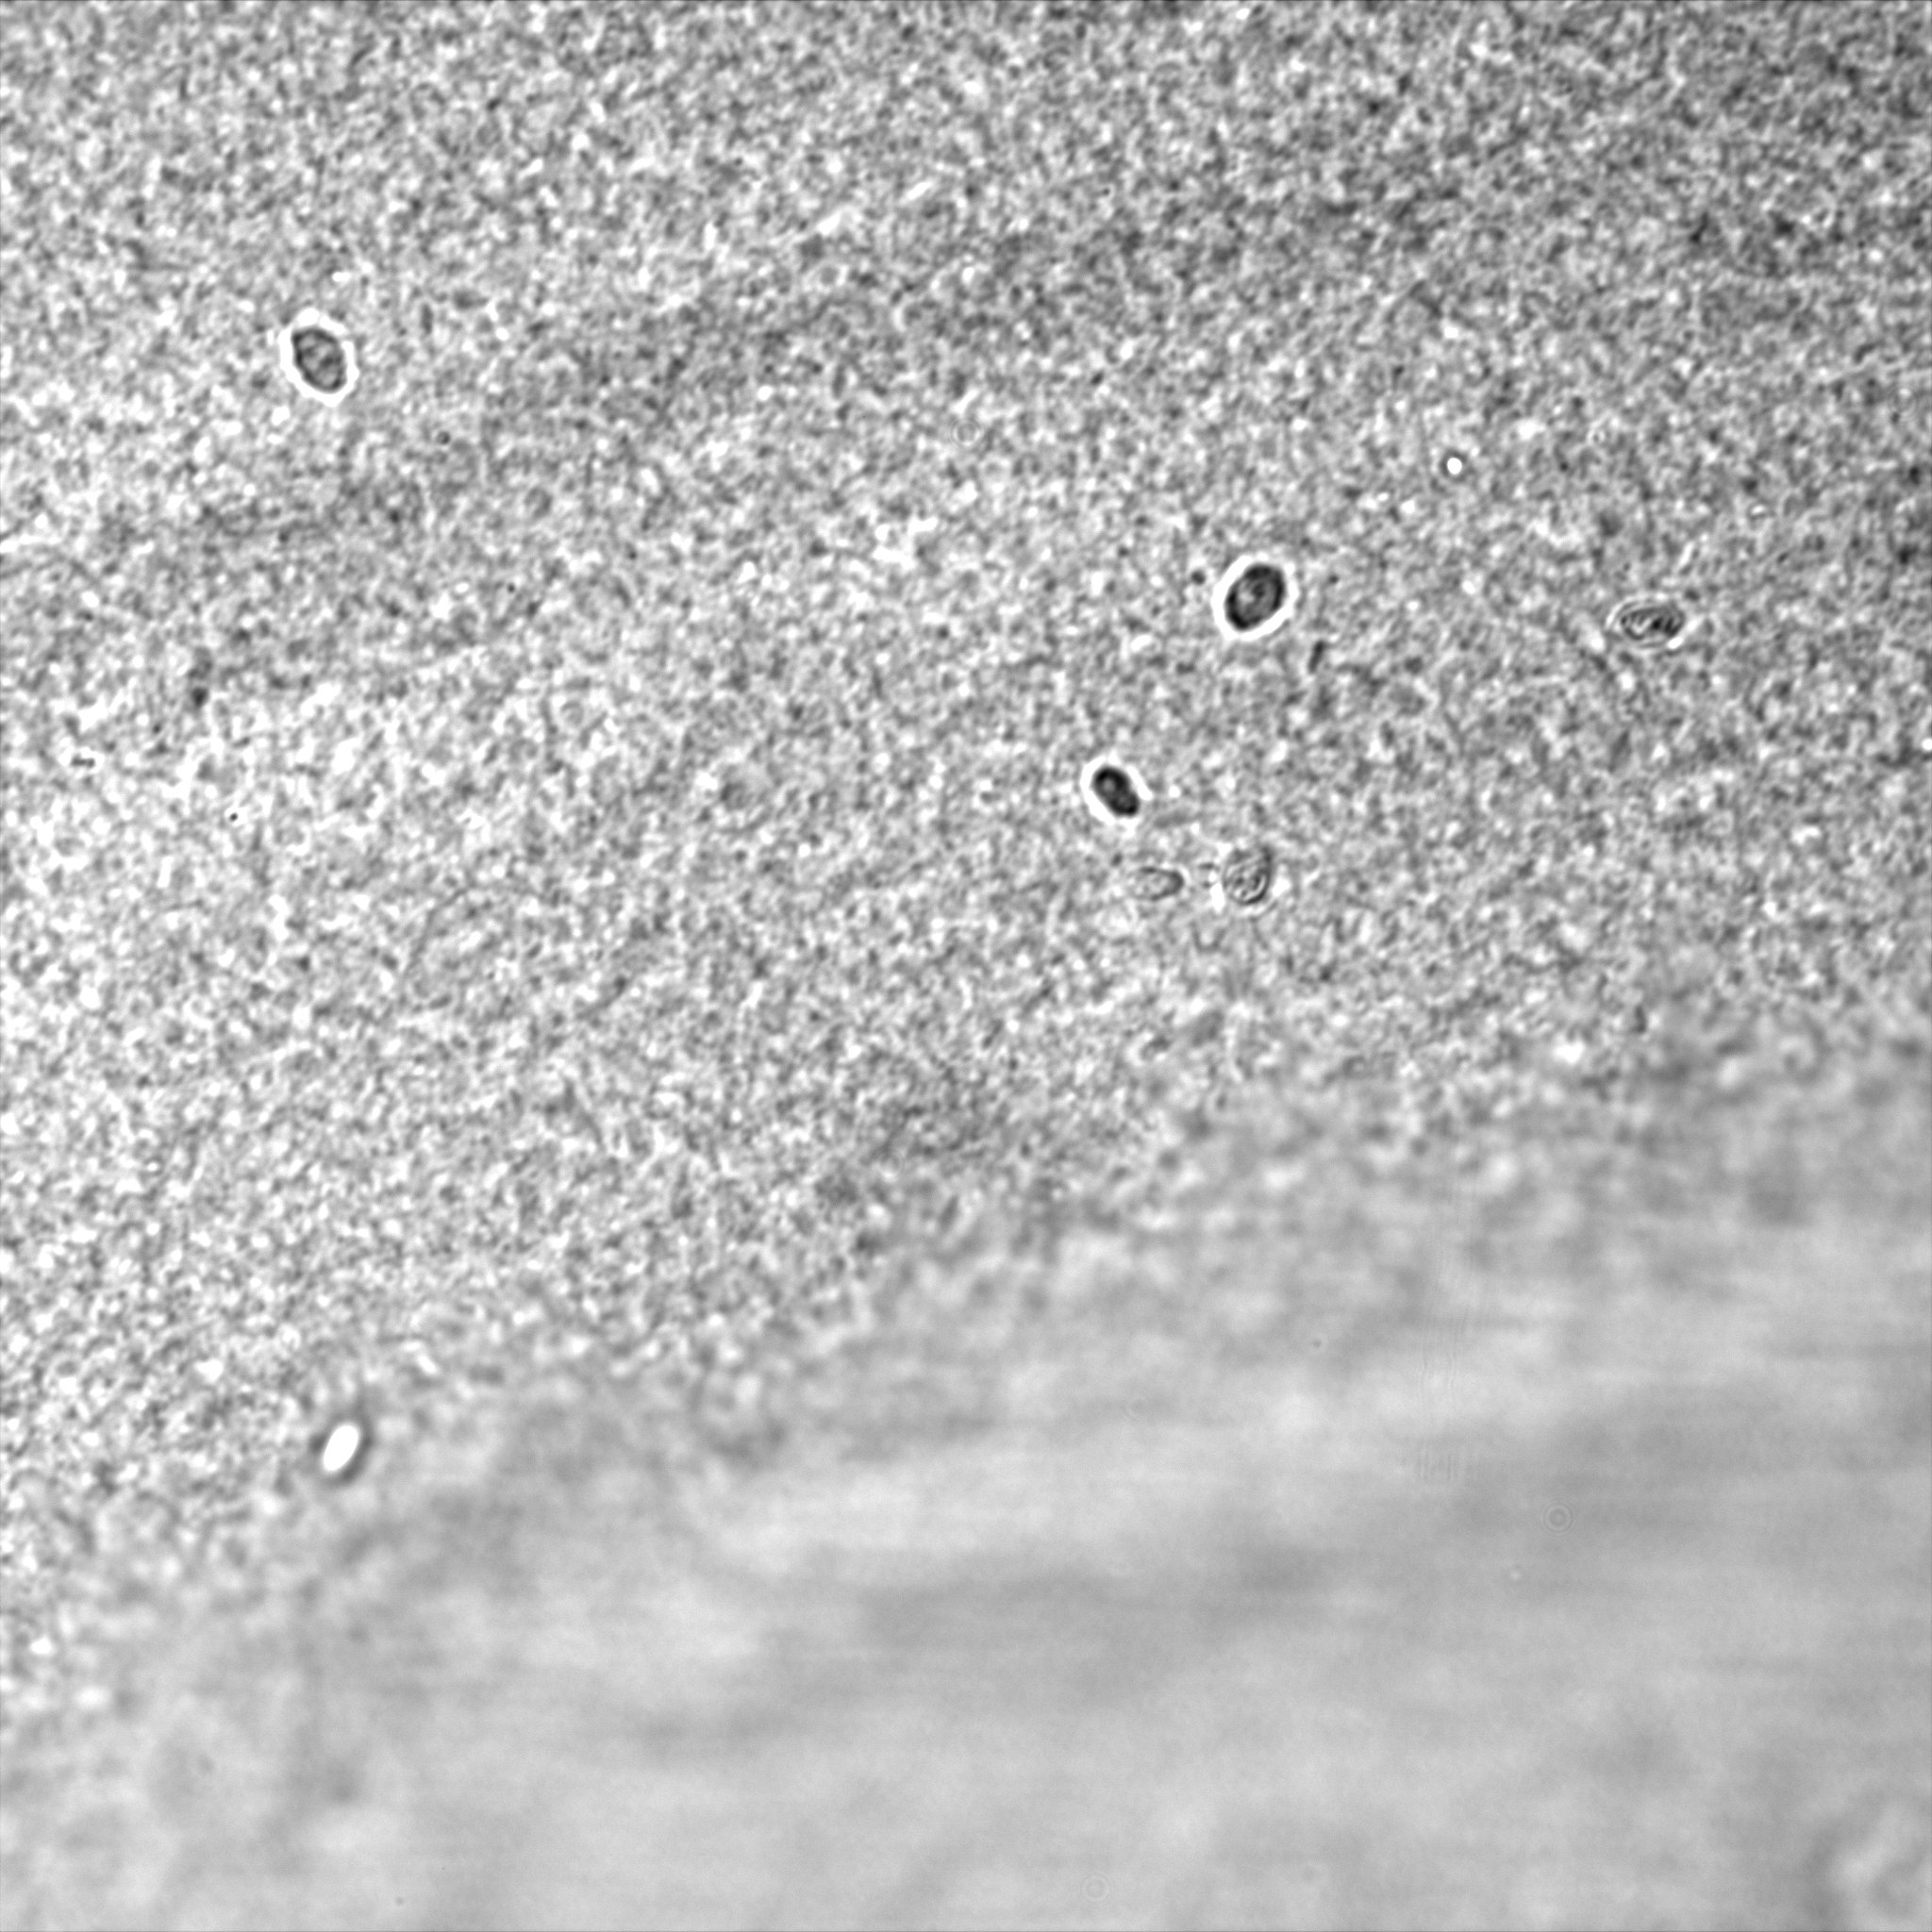
\includegraphics[width=0.3\textwidth]{fracture2_z=0um.jpg}&%
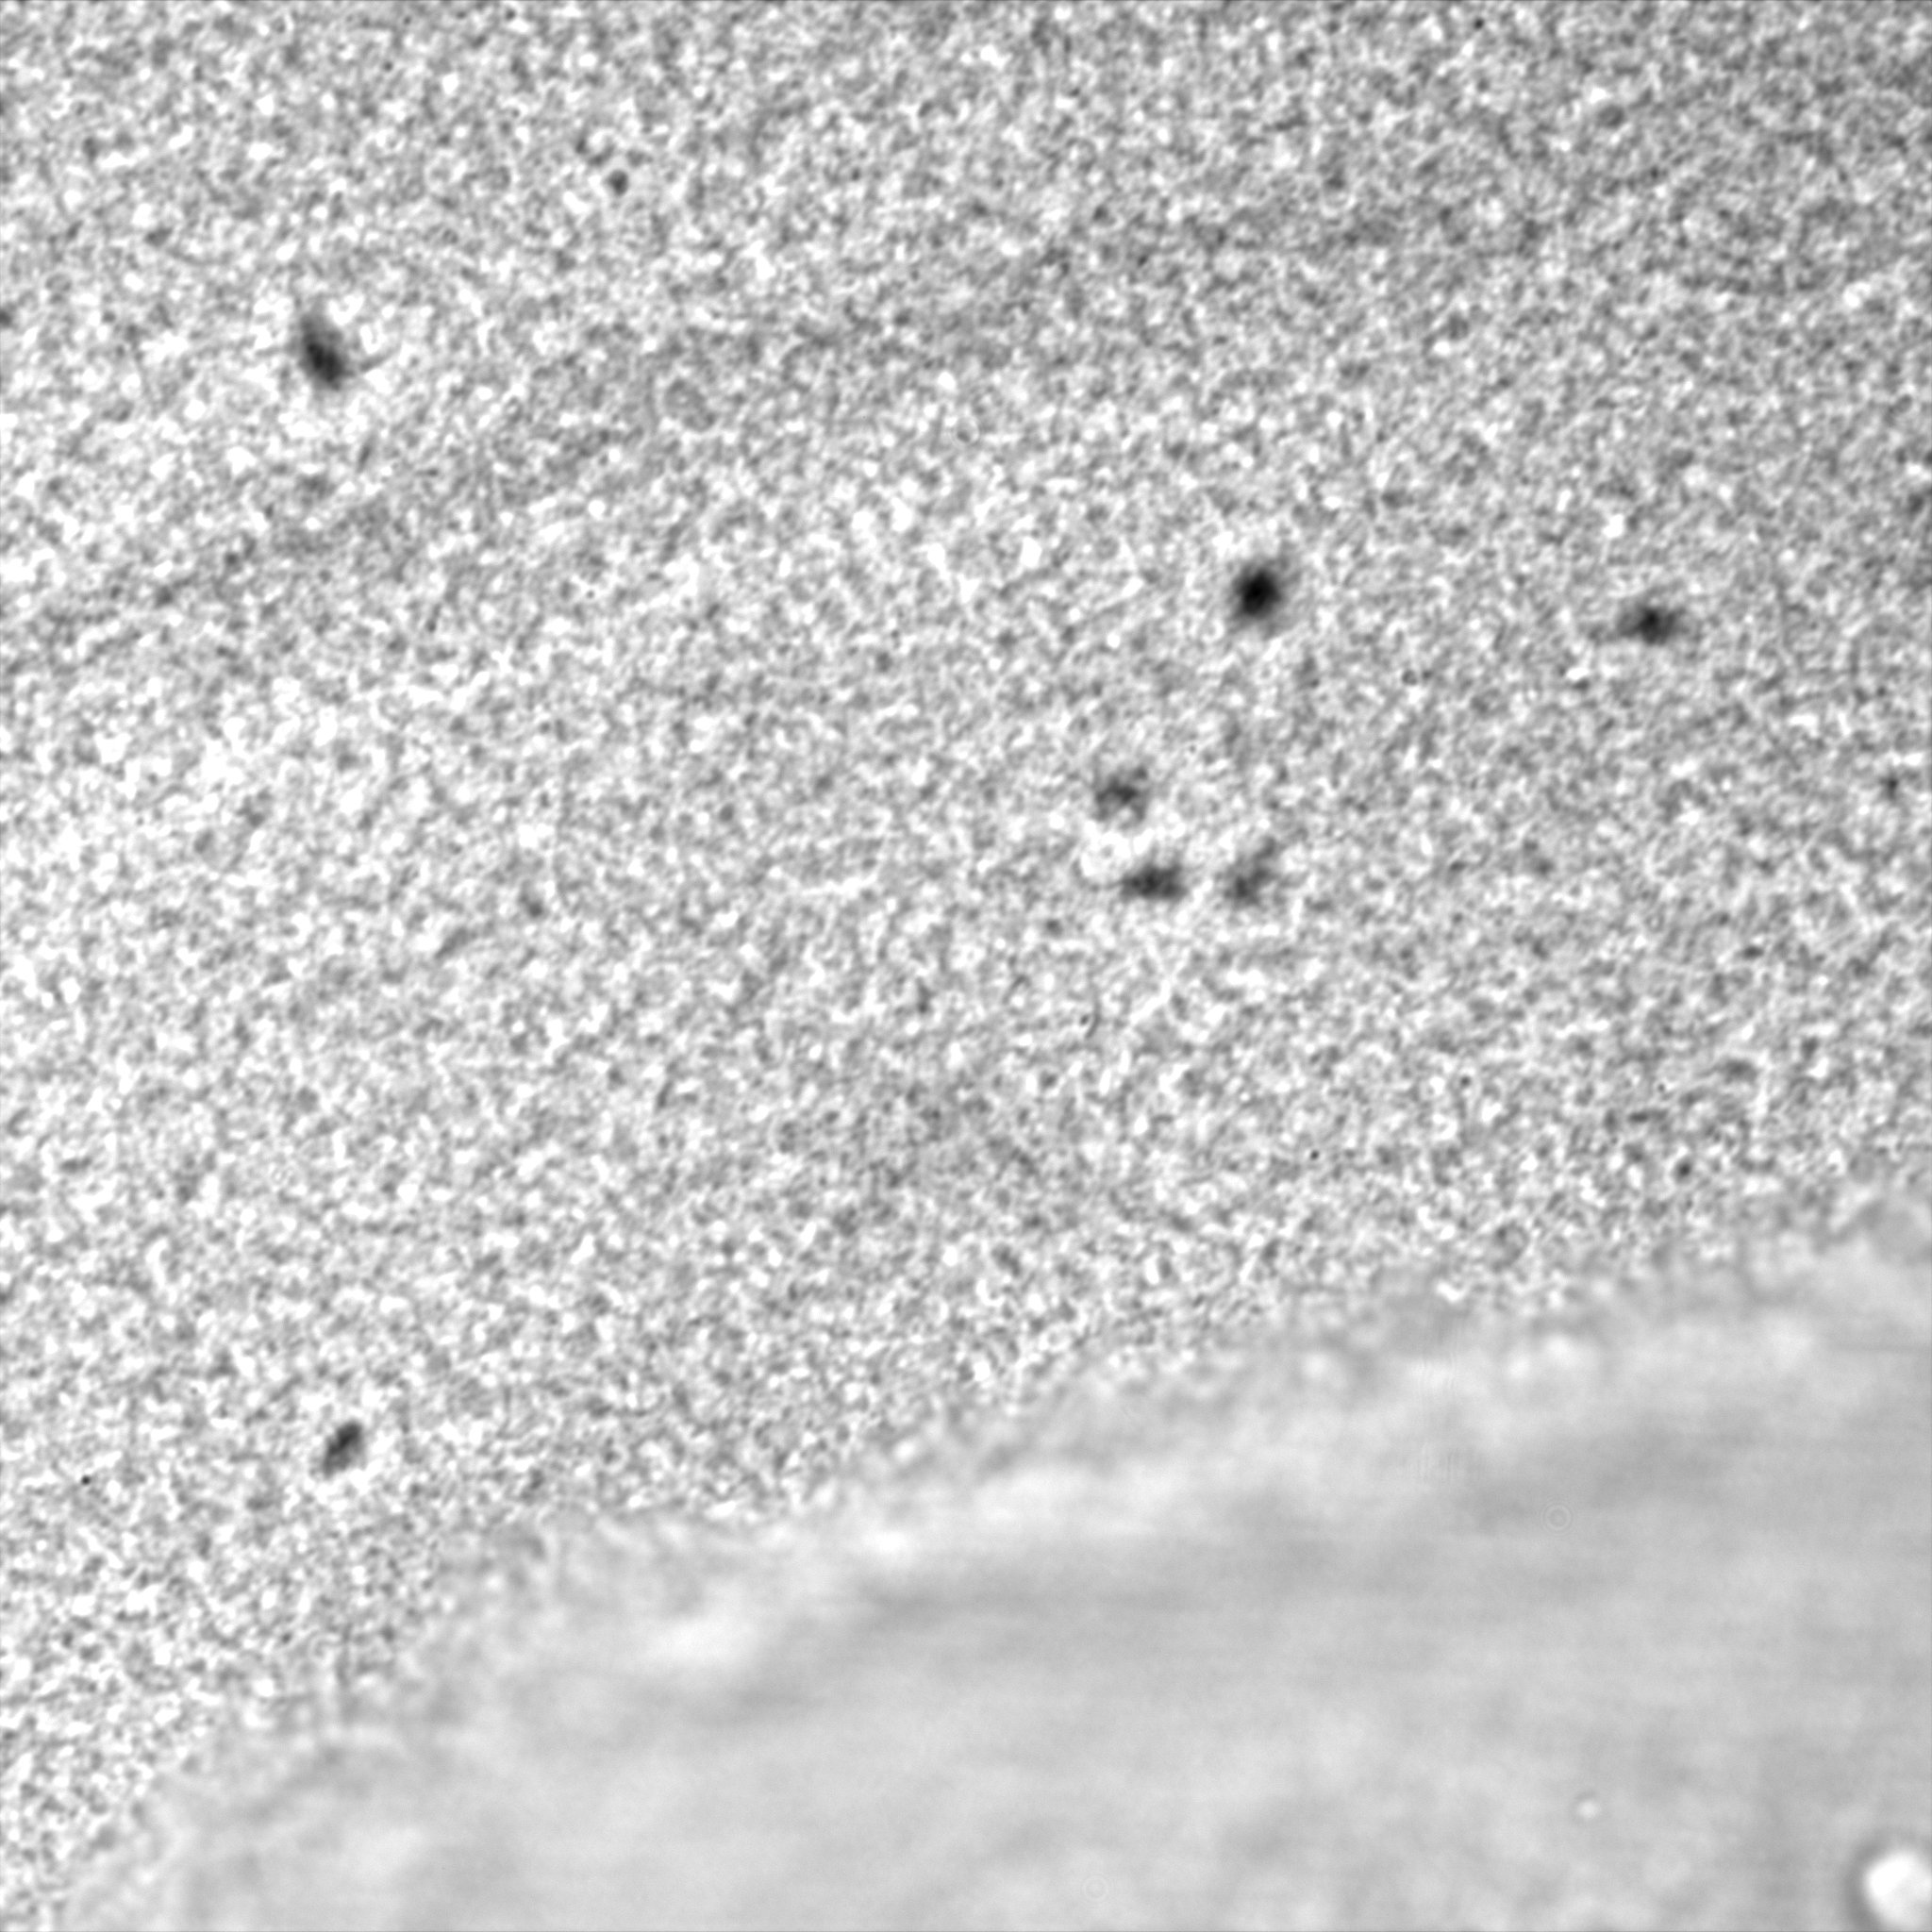
\includegraphics[width=0.3\textwidth]{fracture2_z=15um.jpg}&%
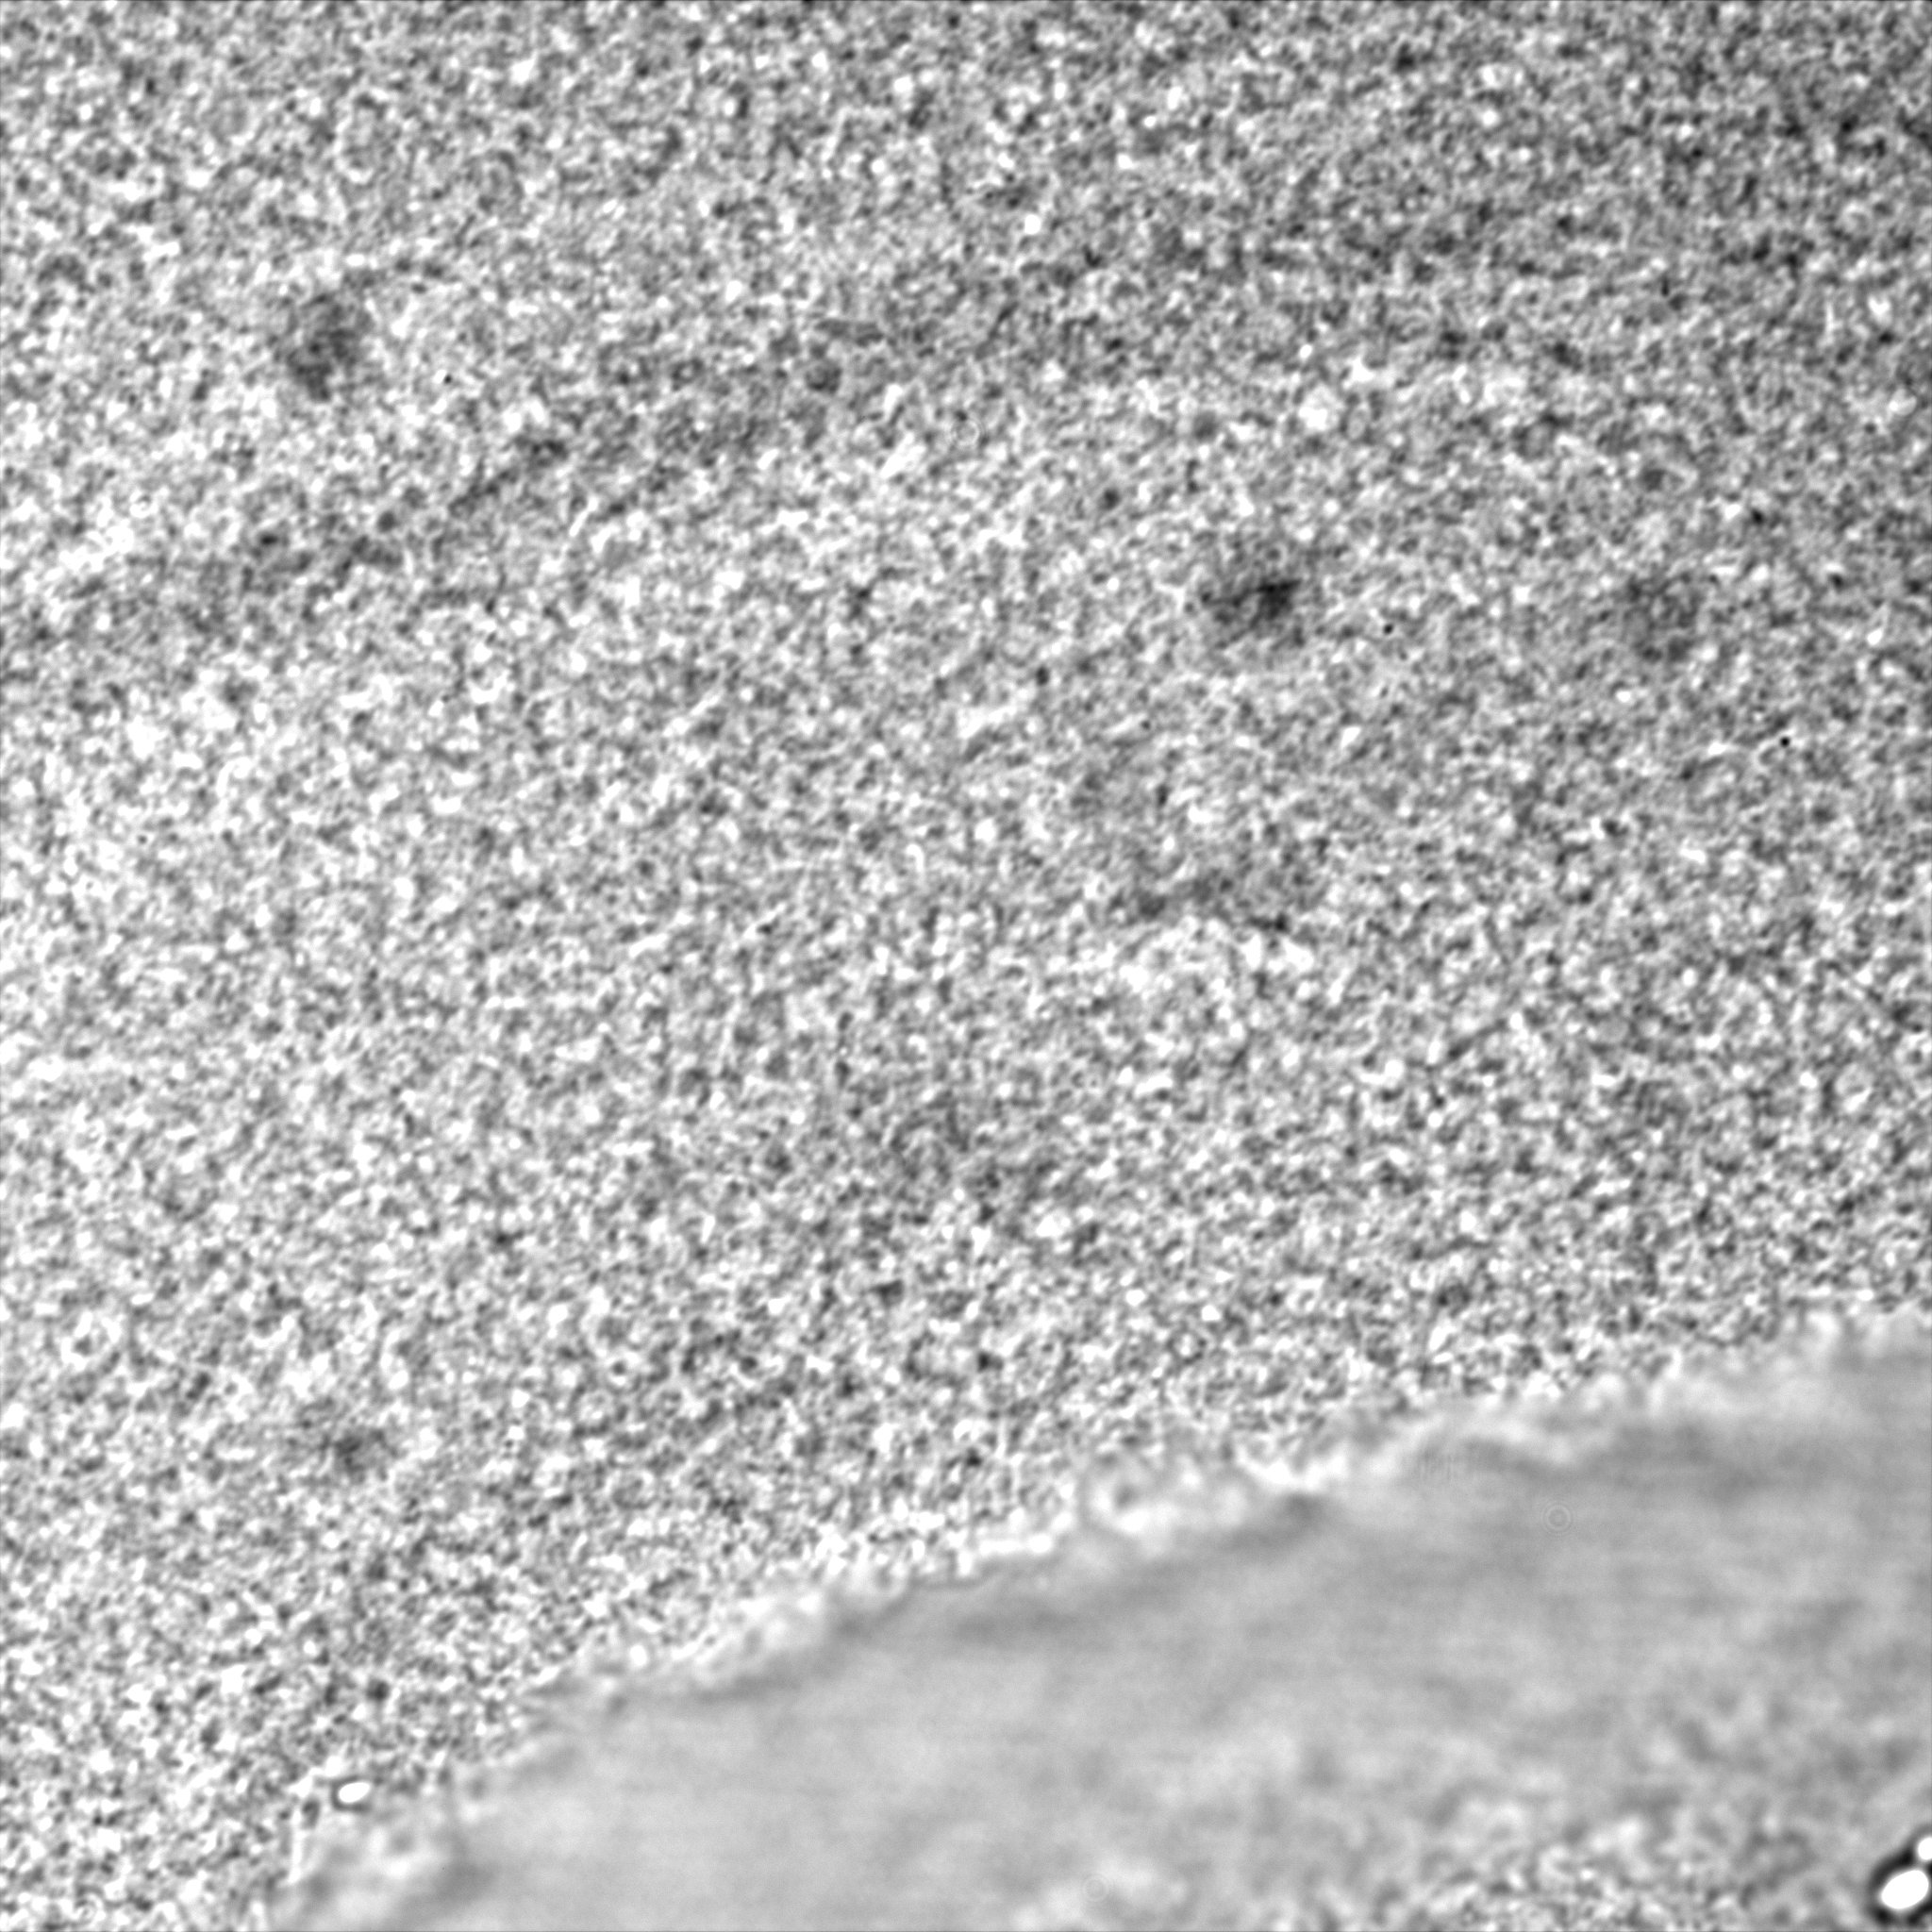
\includegraphics[width=0.3\textwidth]{fracture2_z=30um.jpg}\\
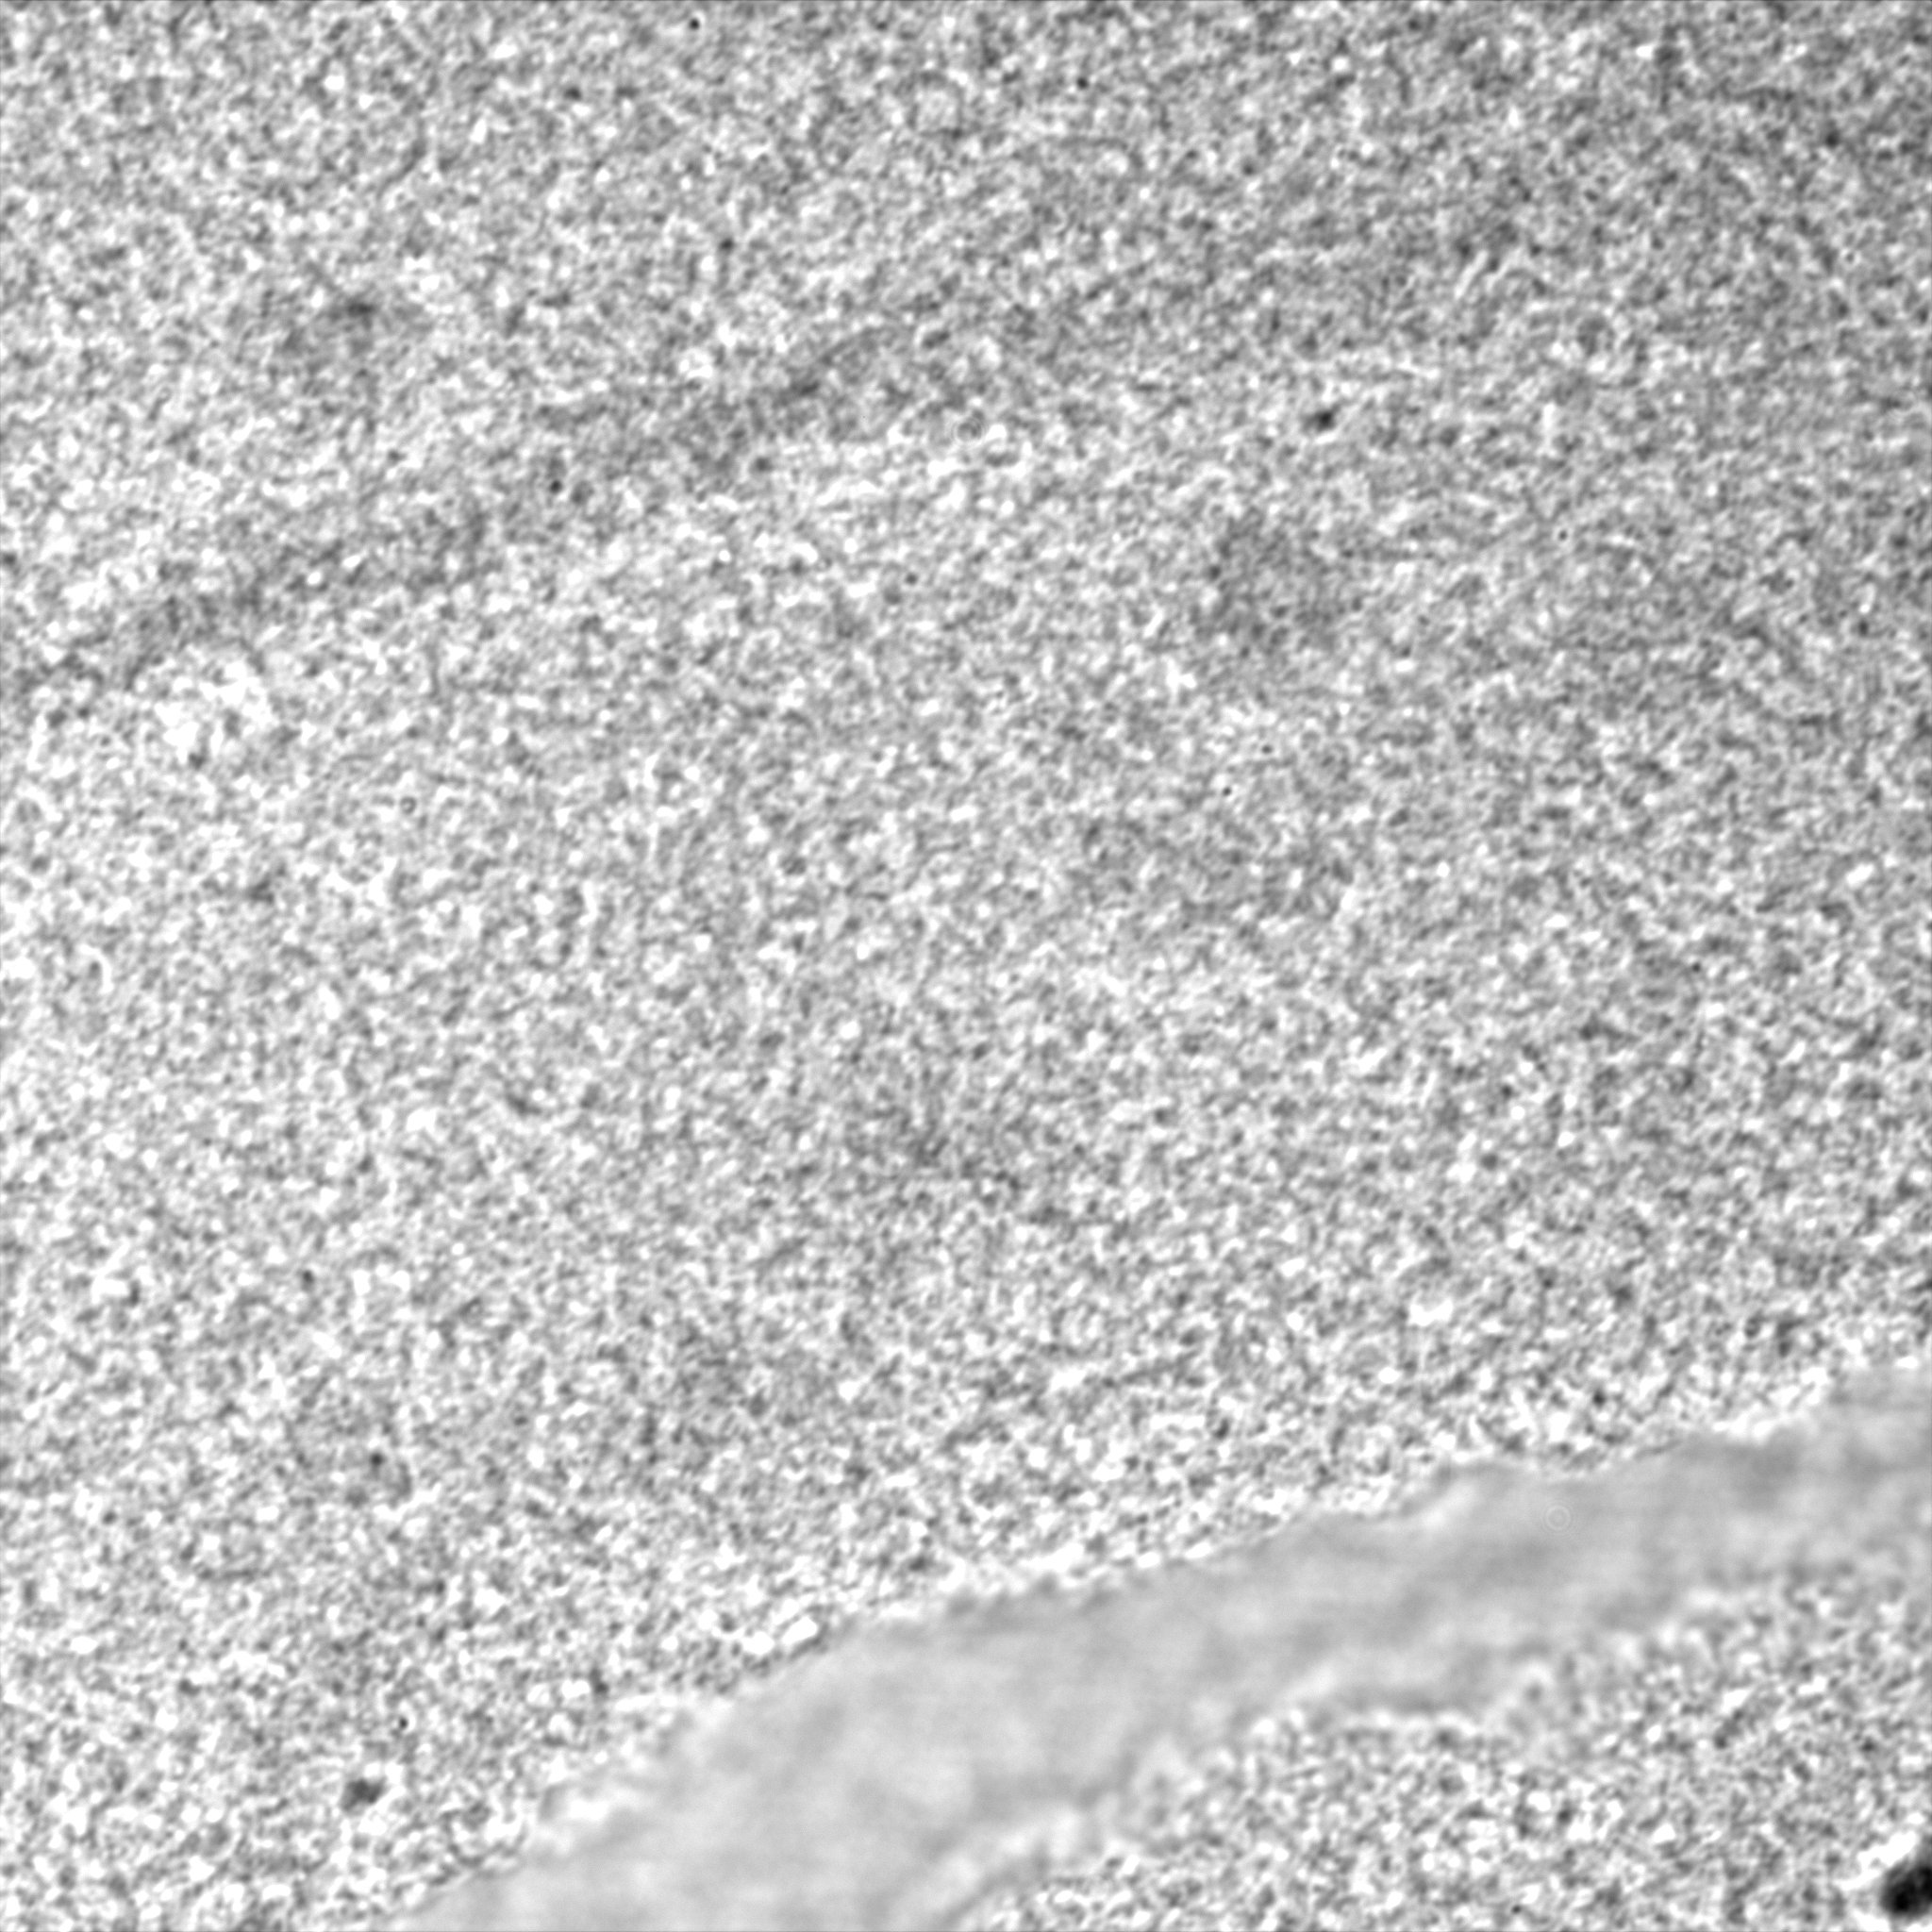
\includegraphics[width=0.3\textwidth]{fracture2_z=45um.jpg}&%
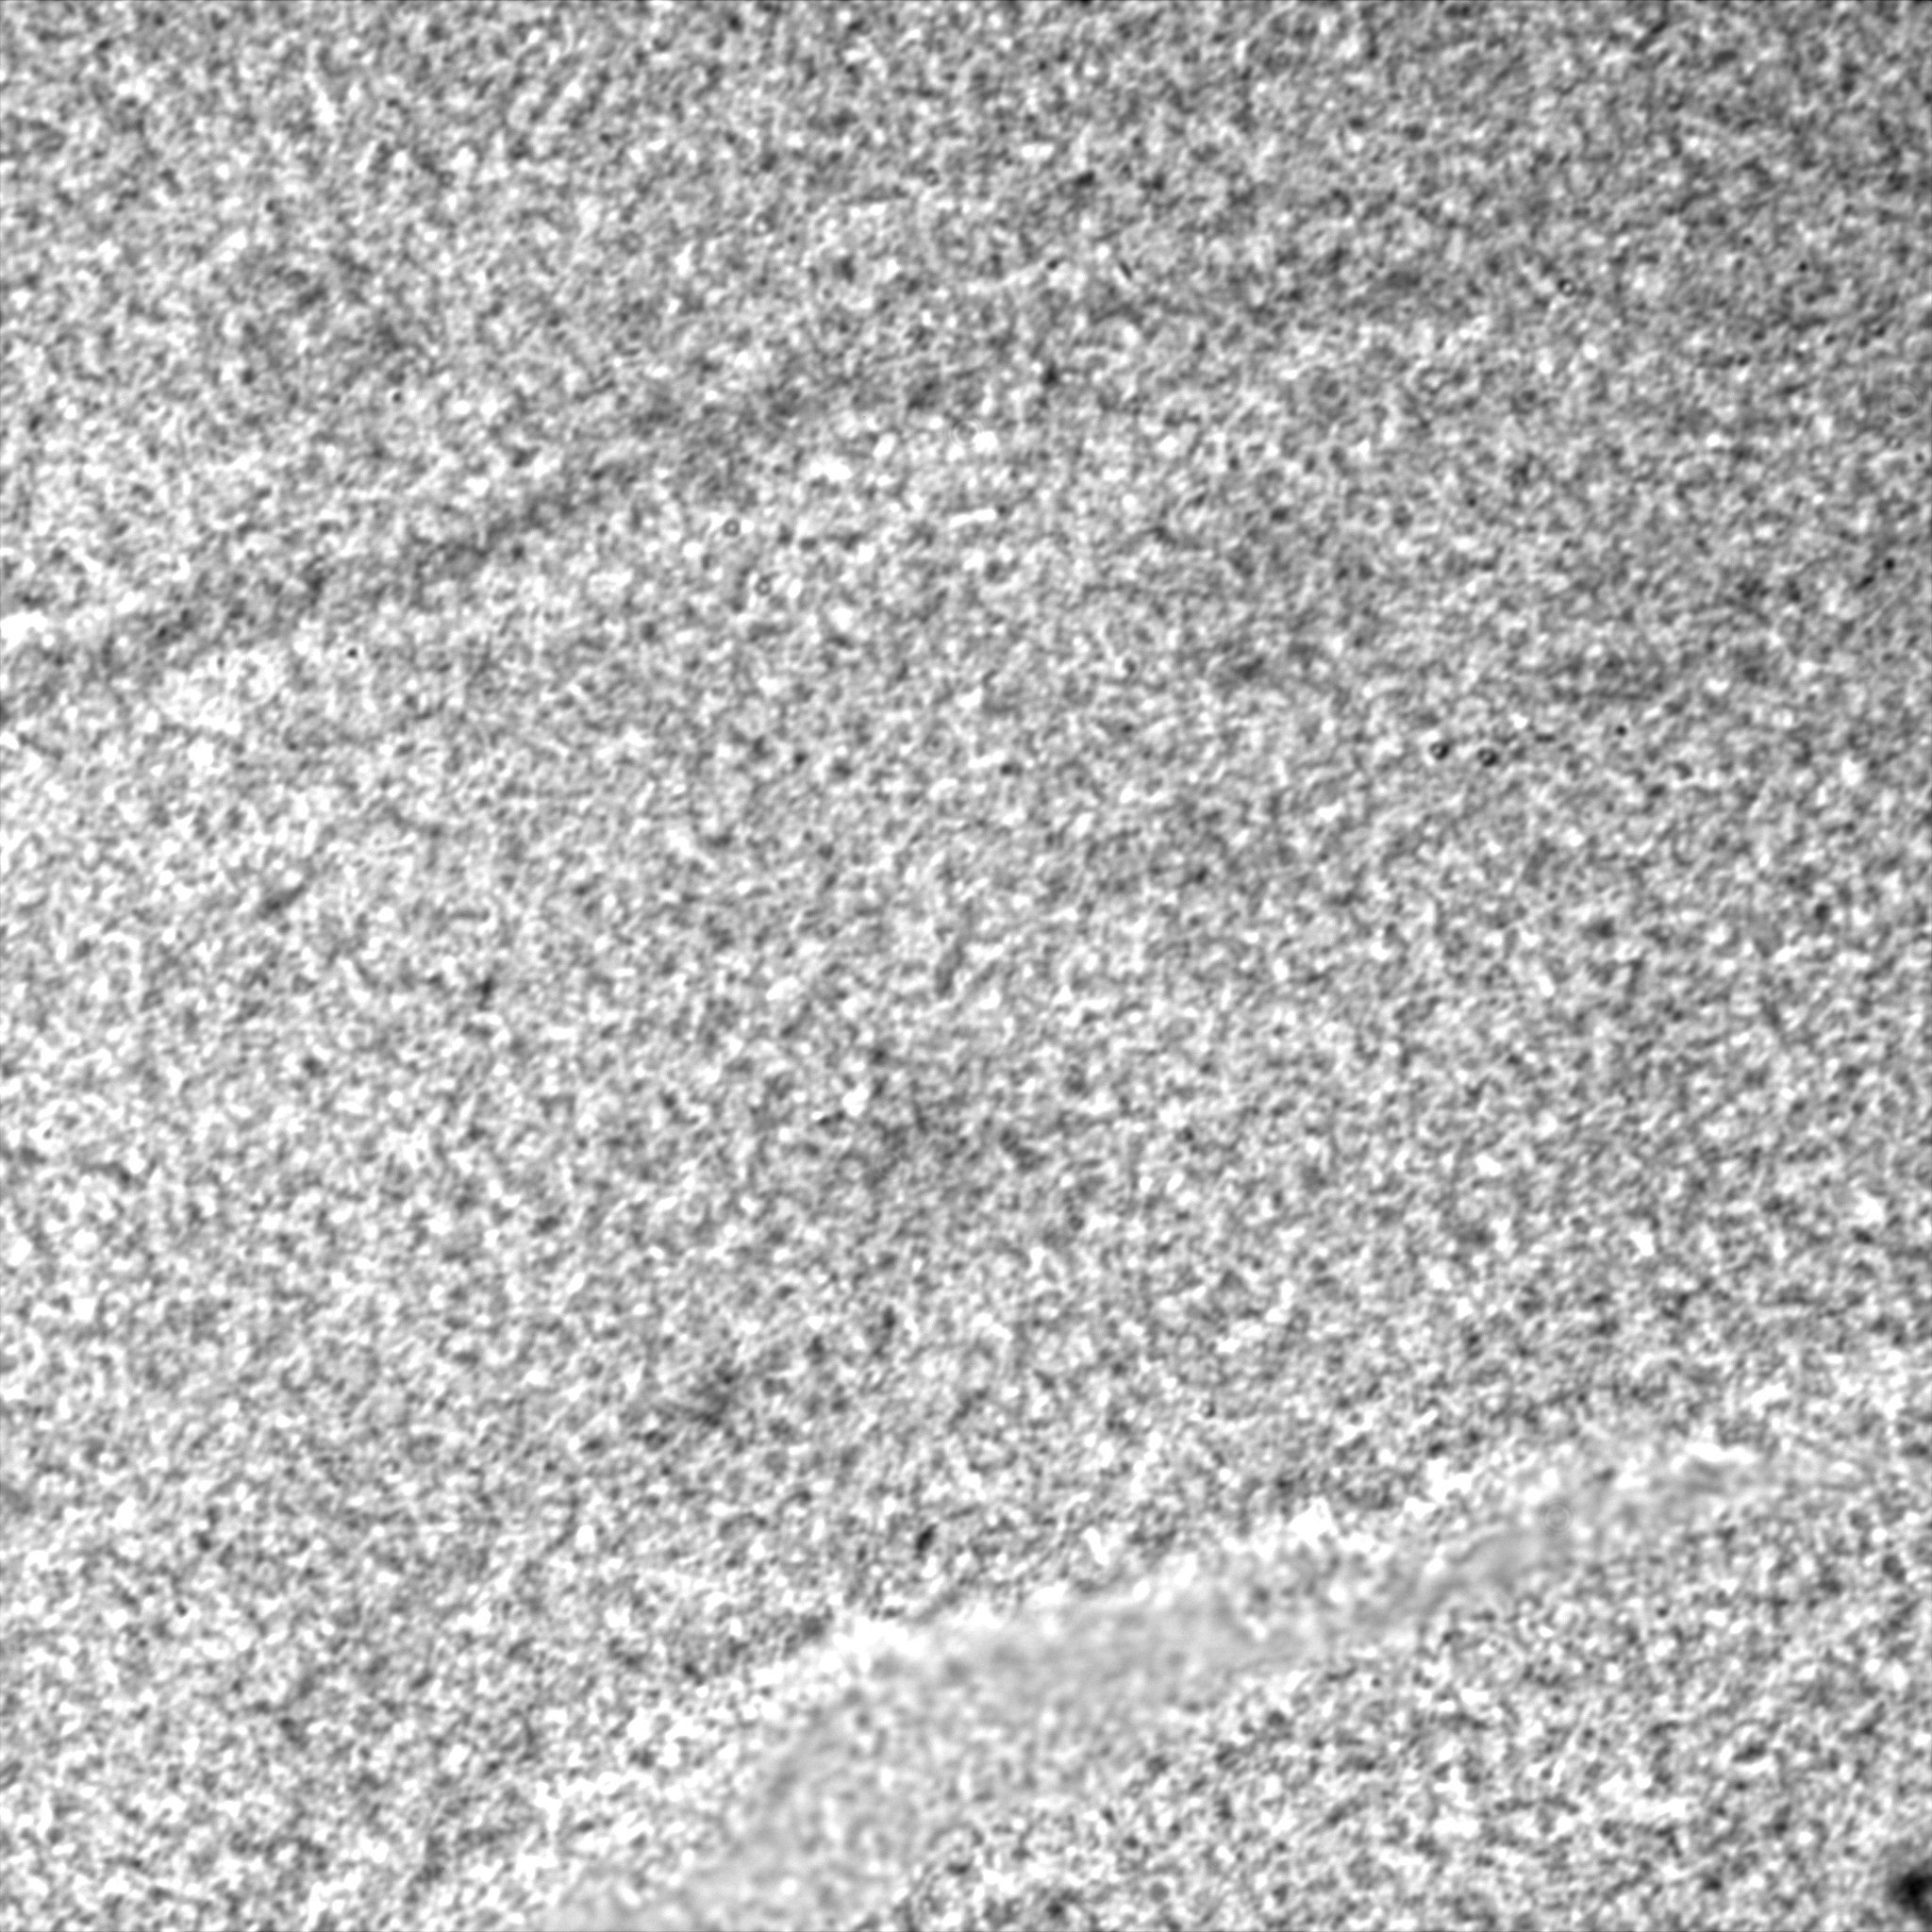
\includegraphics[width=0.3\textwidth]{fracture2_z=60um.jpg}&%
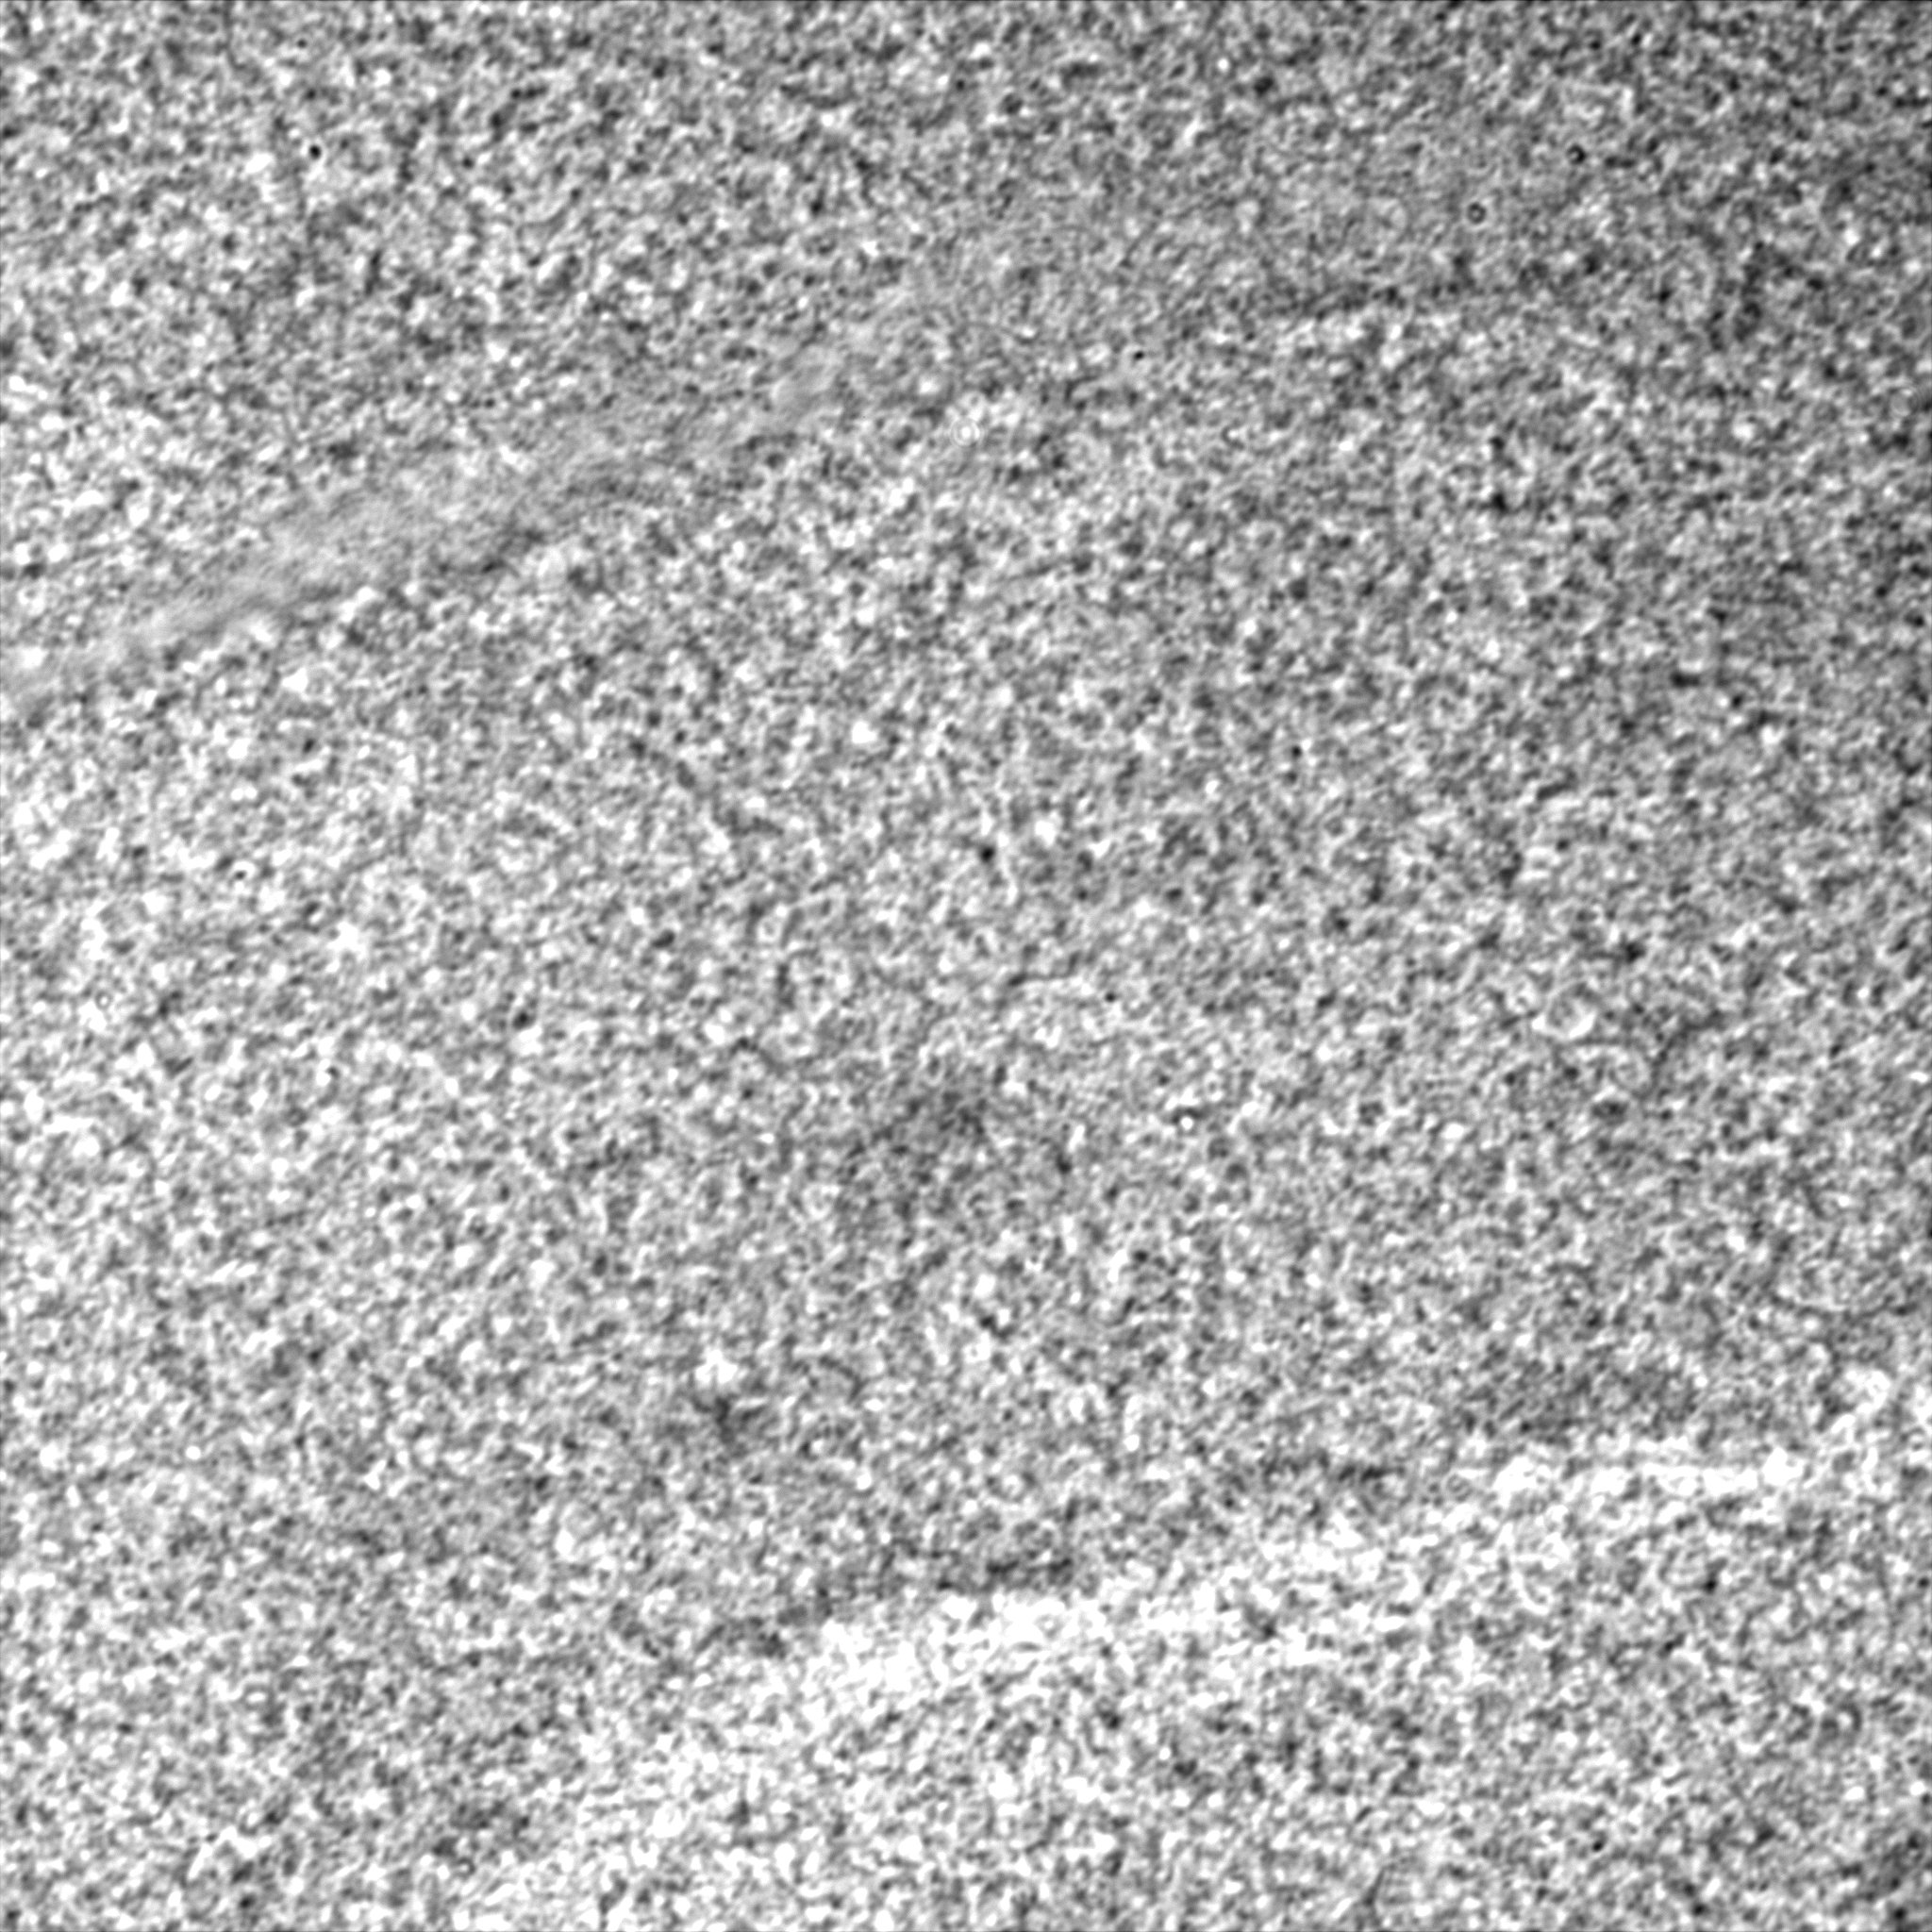
\includegraphics[width=0.3\textwidth]{fracture2_z=75um.jpg}\\
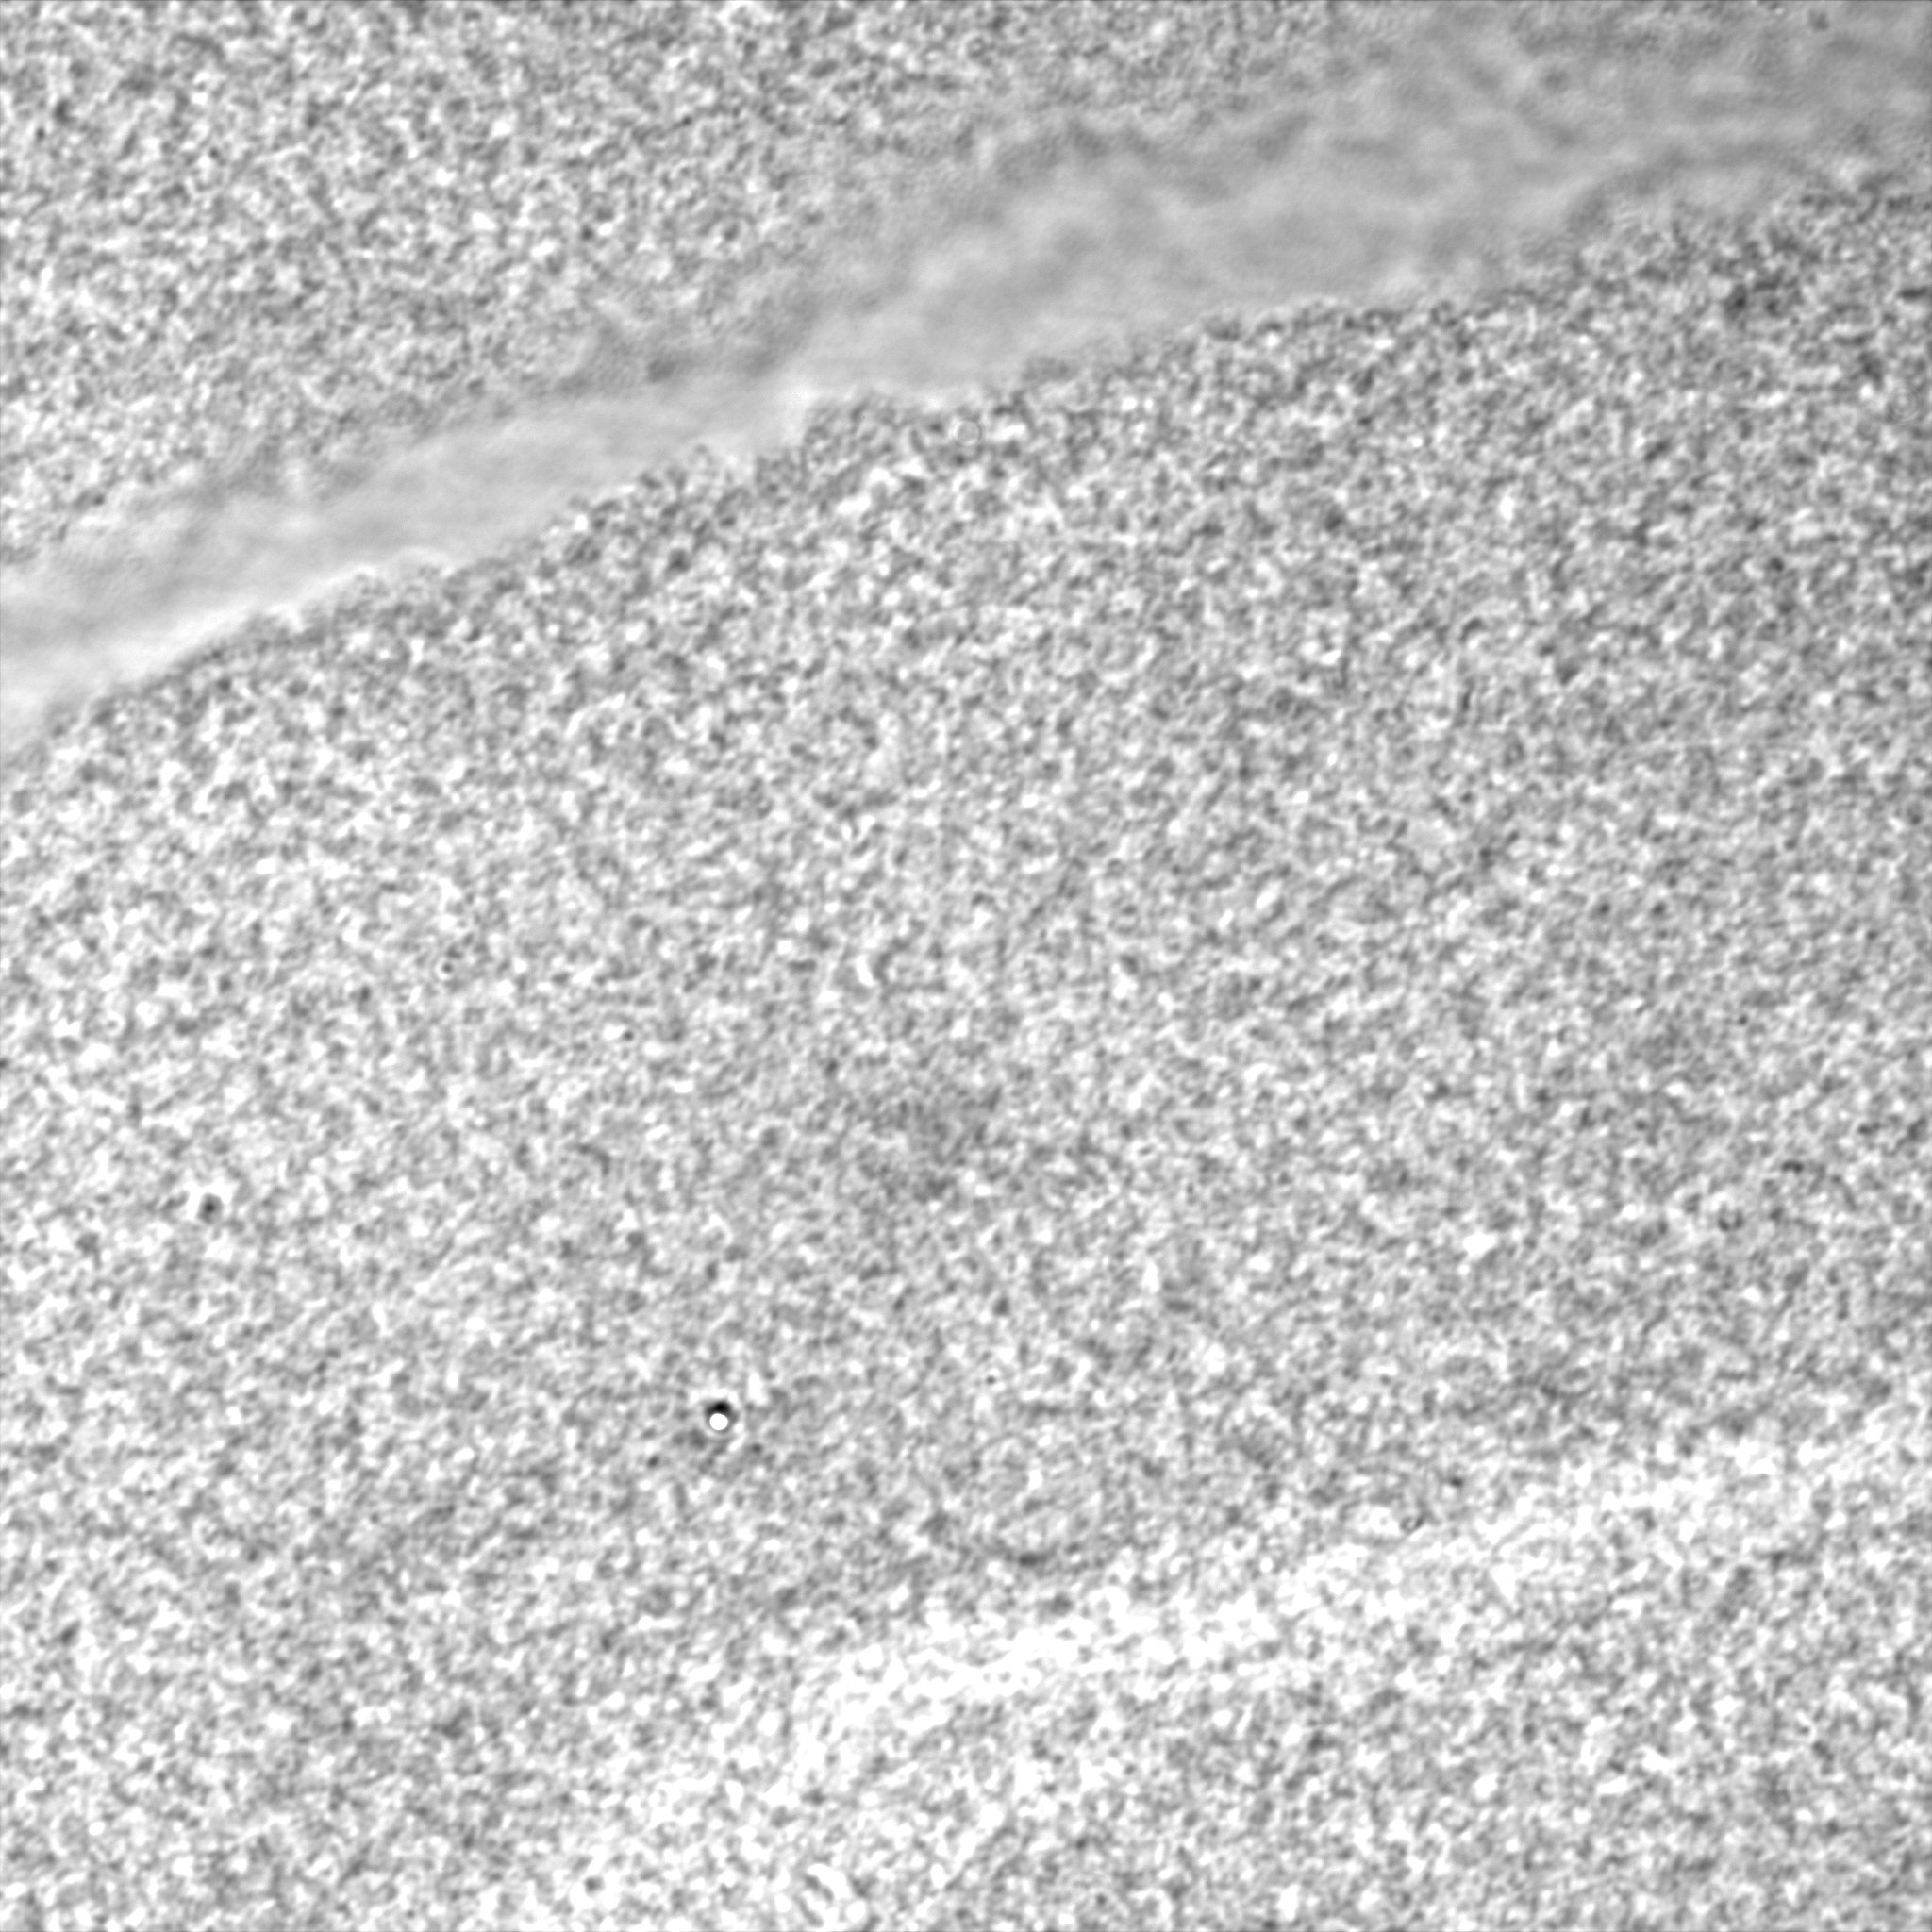
\includegraphics[width=0.3\textwidth]{fracture2_z=90um.jpg}&%
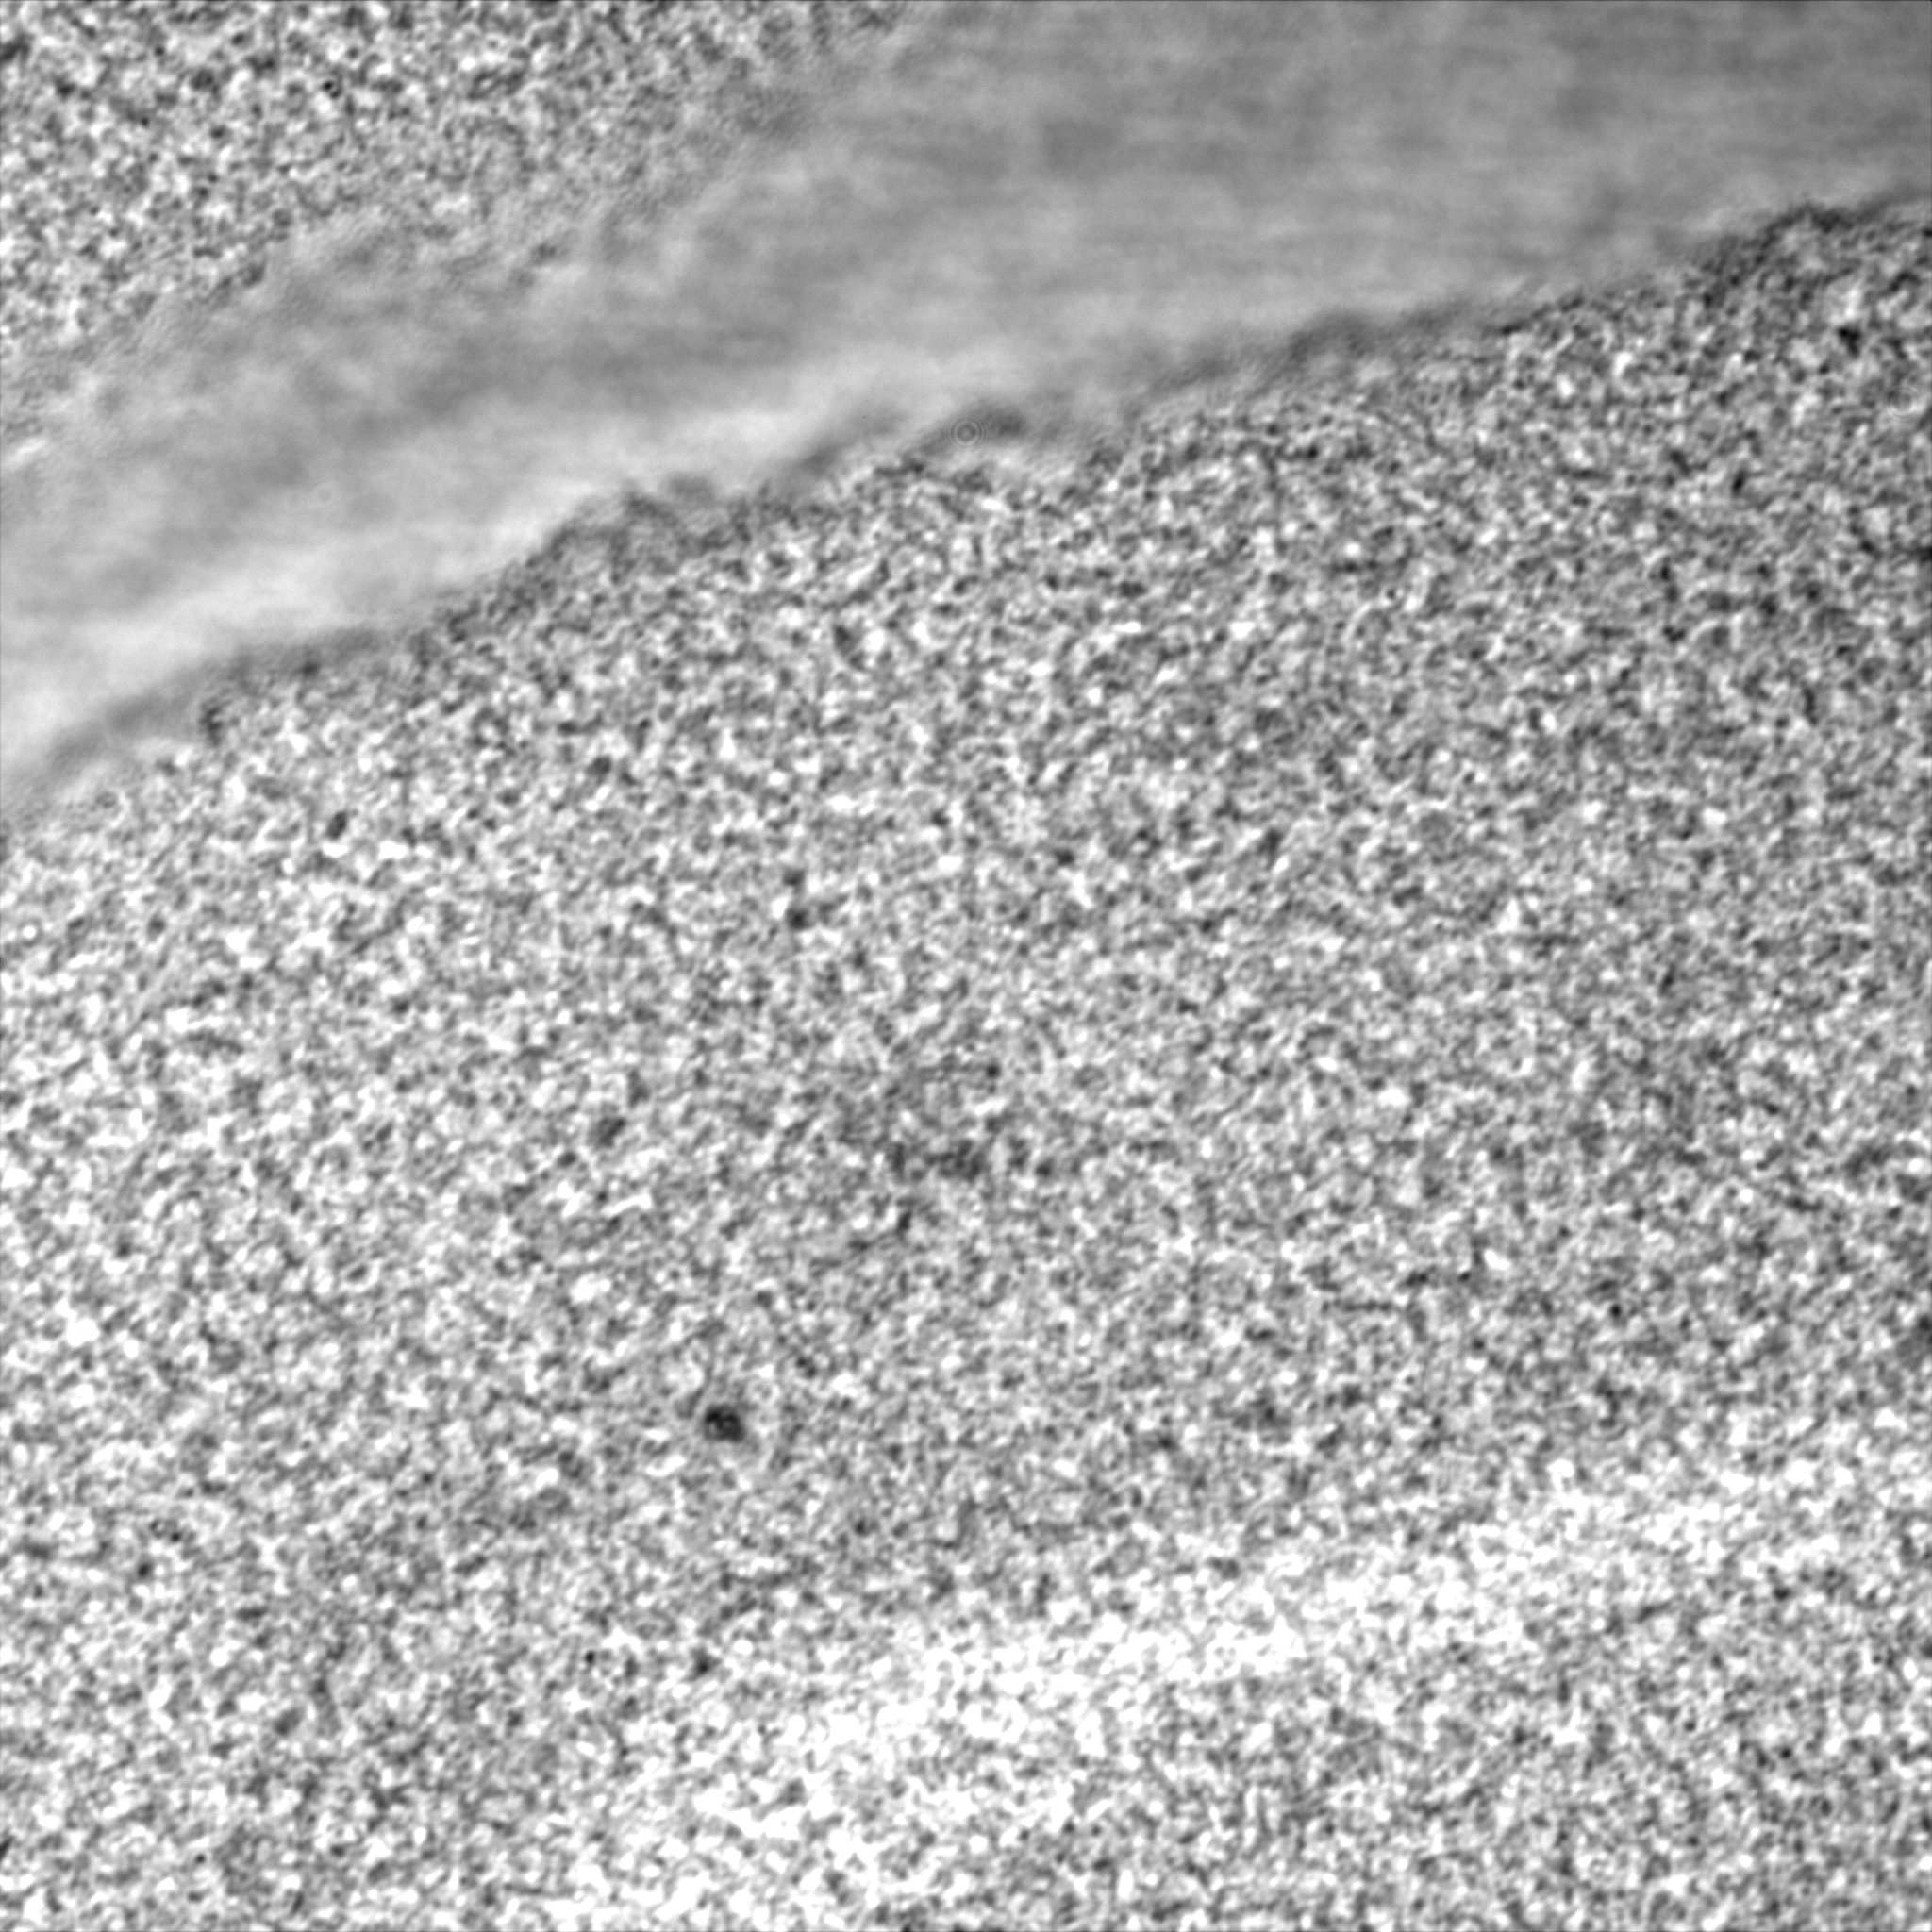
\includegraphics[width=0.3\textwidth]{fracture2_z=105um.jpg}&%
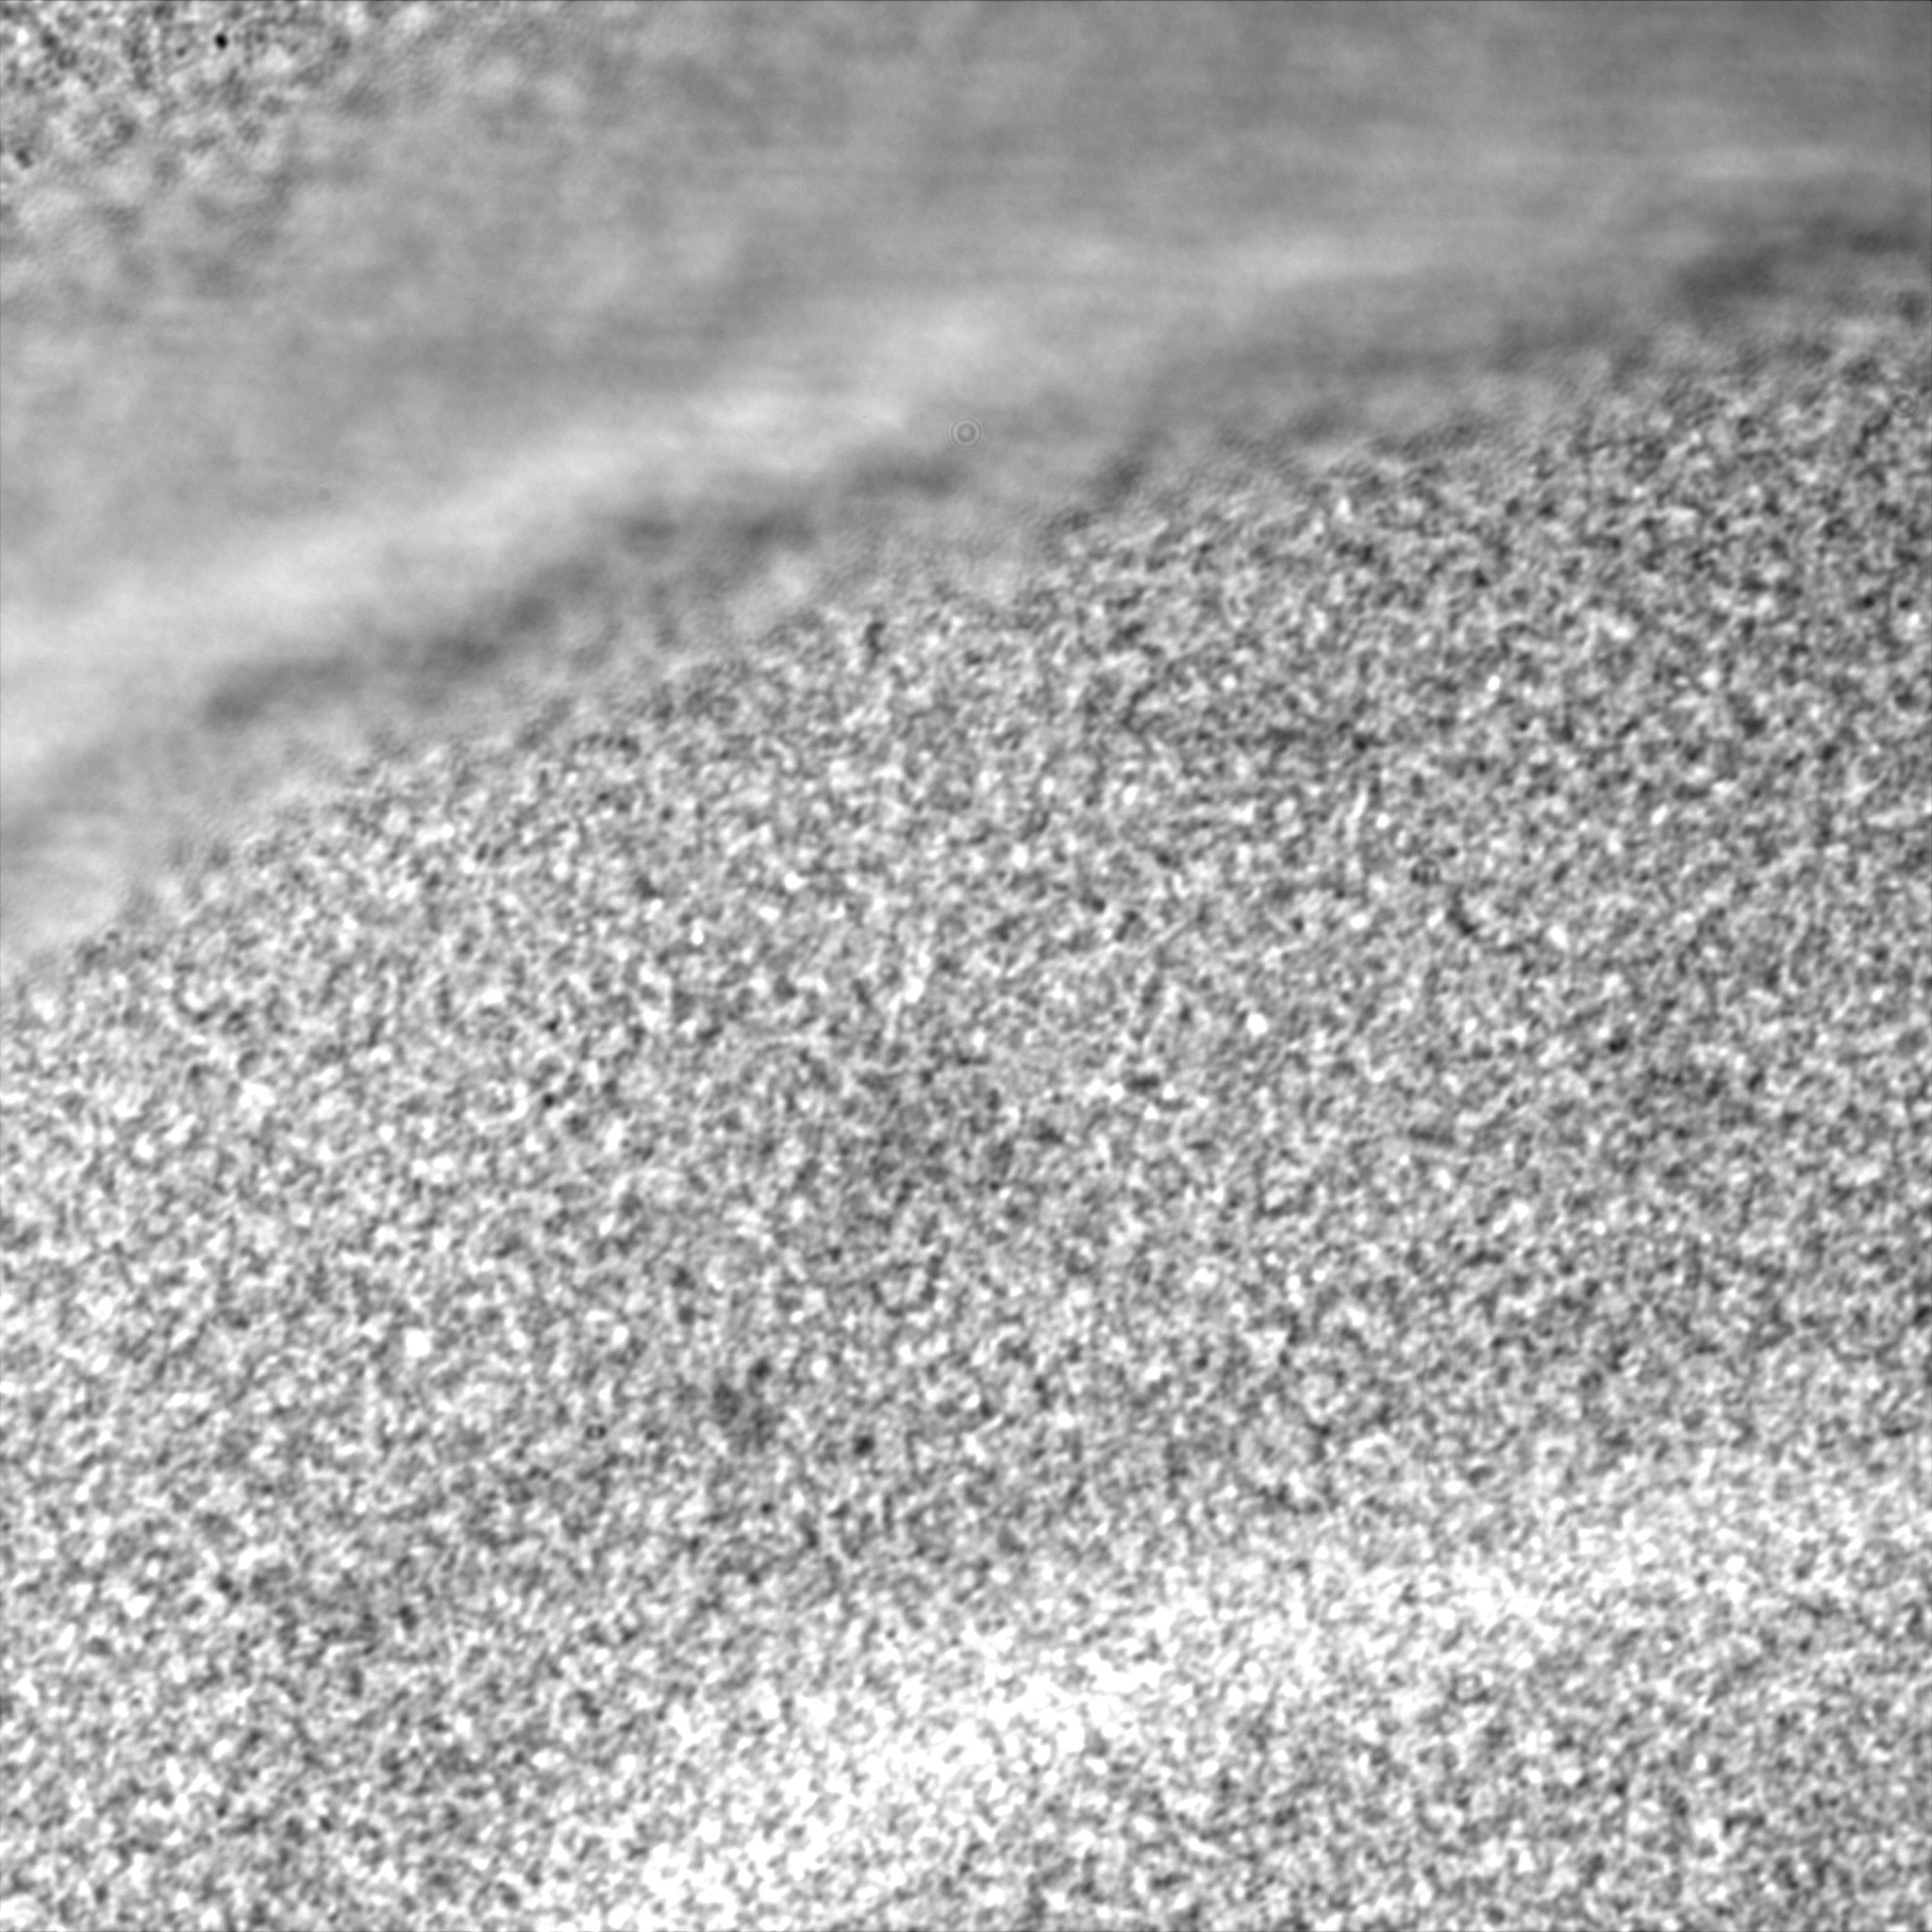
\includegraphics[width=0.3\textwidth]{fracture2_z=120um.jpg}\\
\end{tabular} 
\column{0.3\textwidth}
\begin{tikzpicture}[inner sep=0]
\node{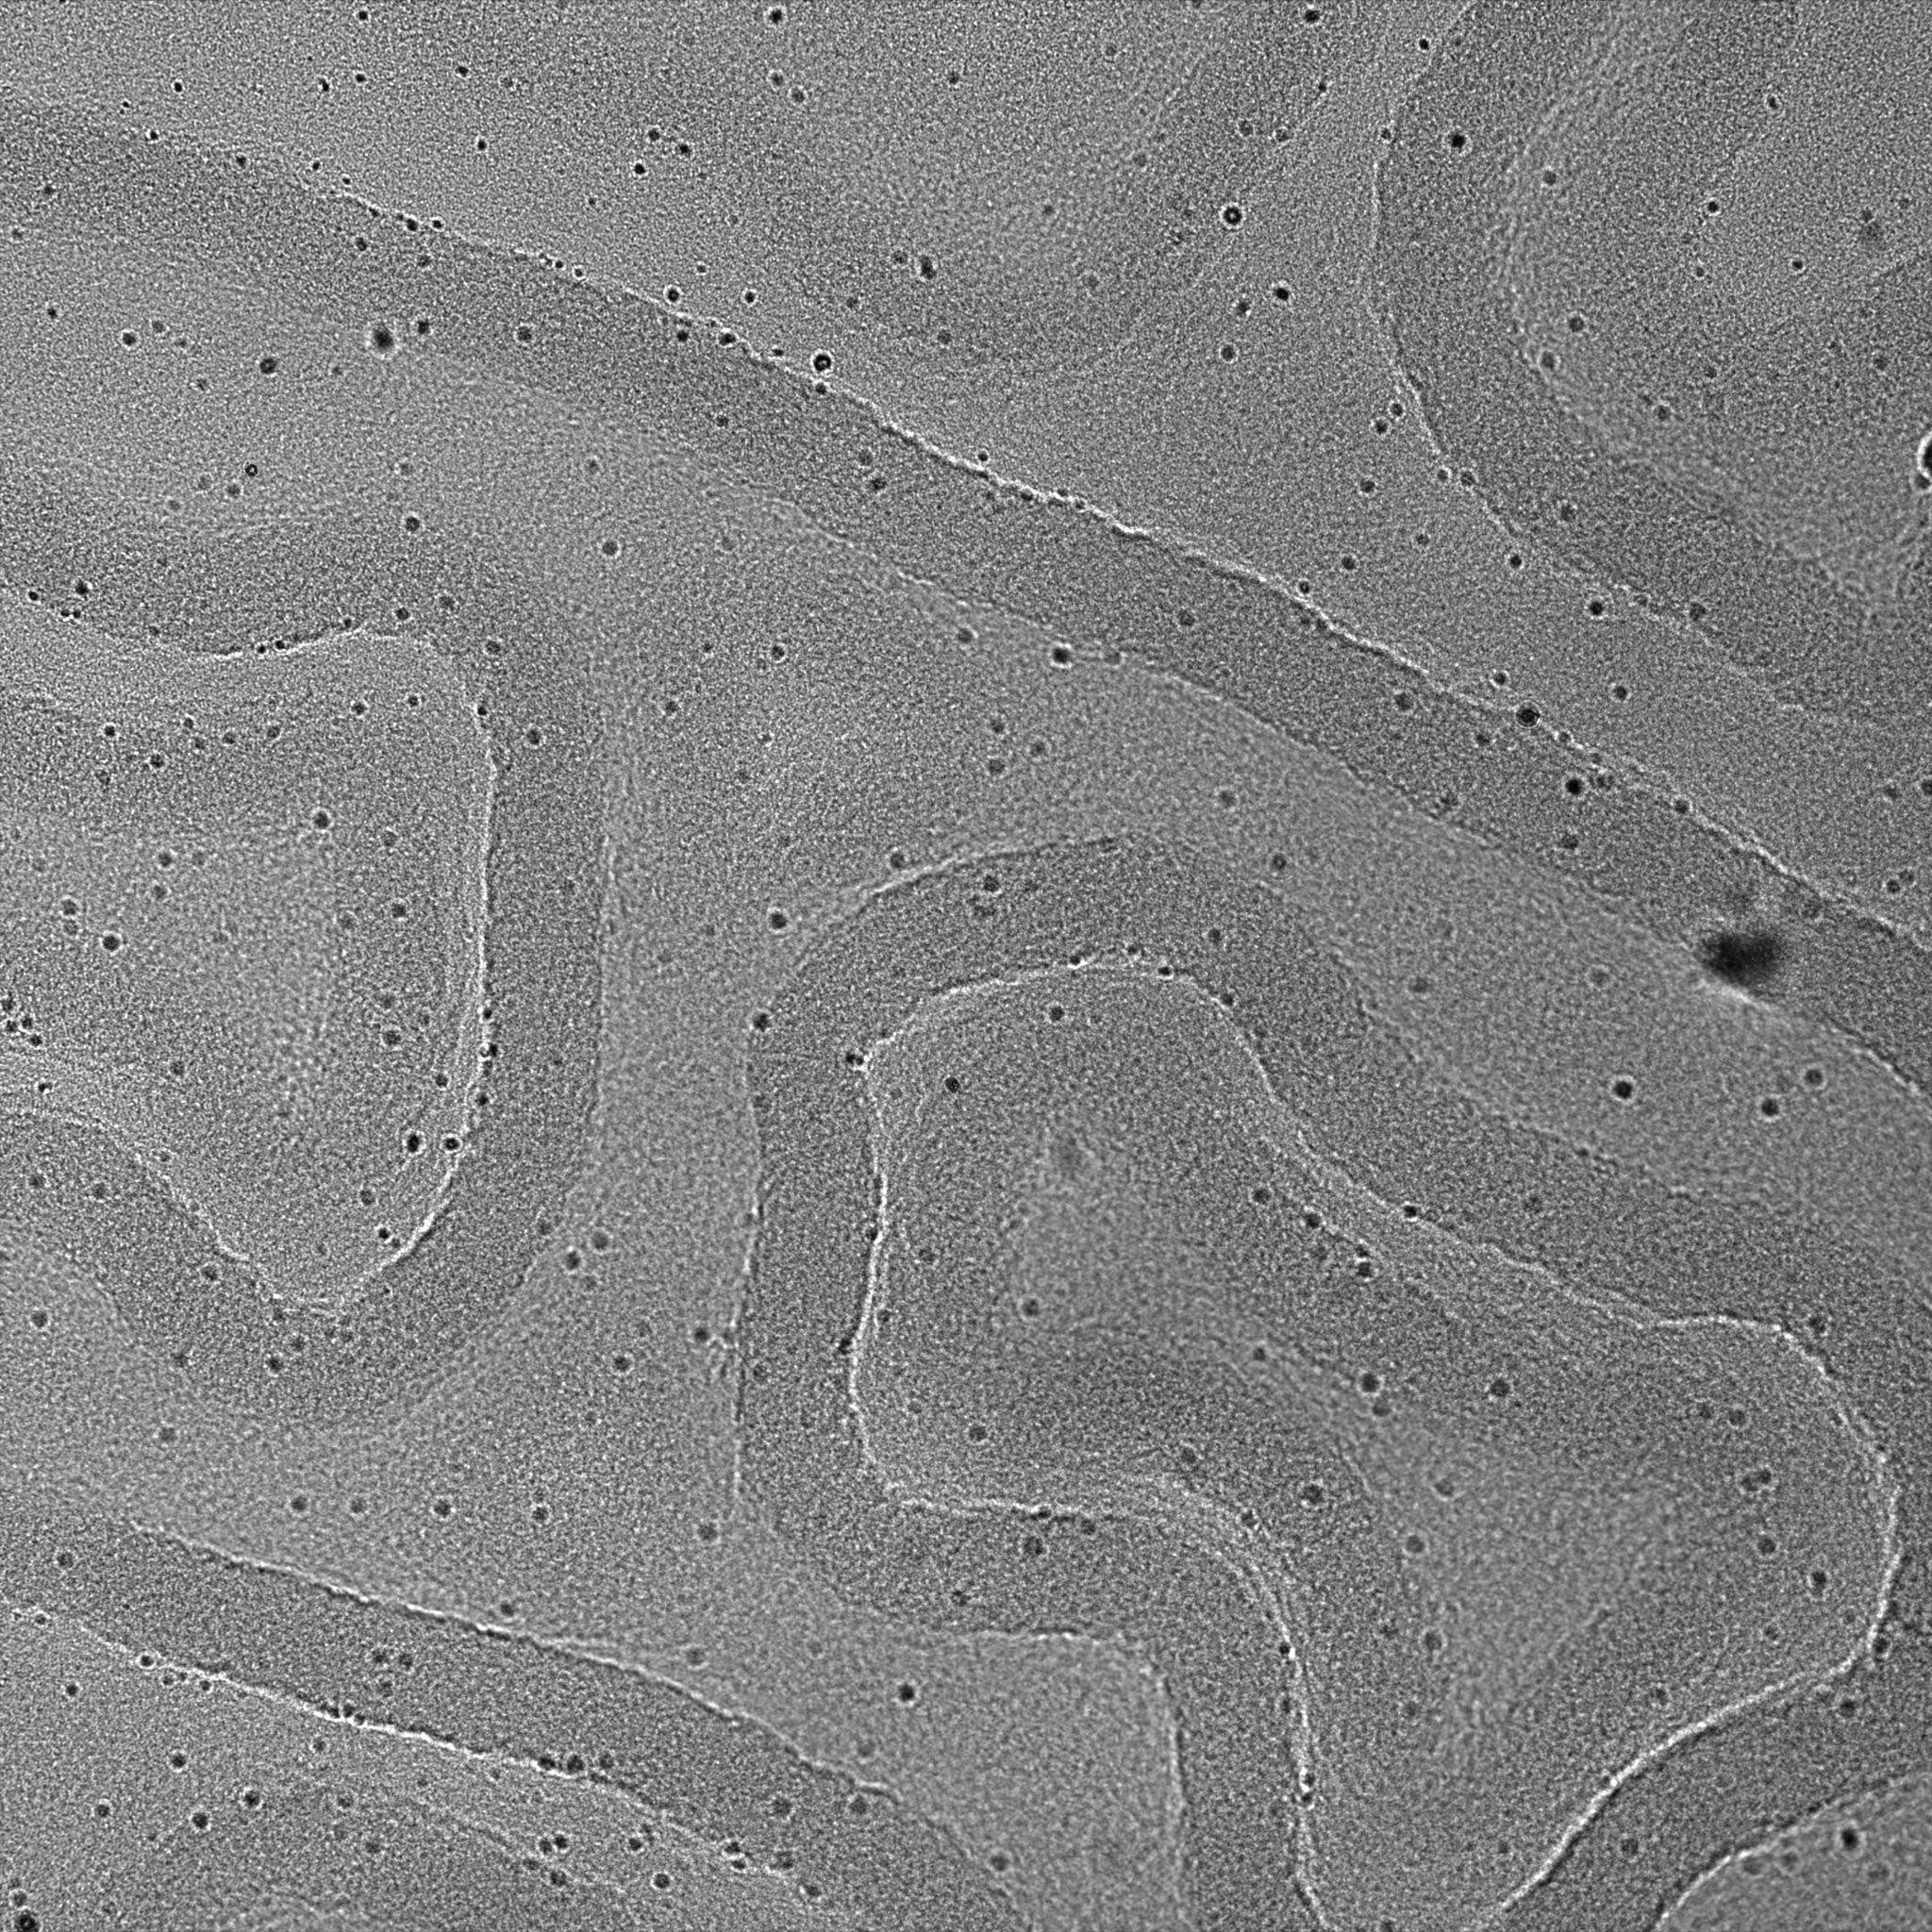
\includegraphics[width=\textwidth]{fracture2_x10.jpg}};
\draw[red] (-0.05\textwidth, -0.05\textwidth) rectangle (0.05\textwidth, 0.05\textwidth);
\end{tikzpicture}

\bigskip

\begin{tikzpicture}[inner sep=0]
\node{
\includegraphics[width=\textwidth]{coupe_motif.pdf}};
\node[anchor=west] at (-0.45\textwidth, 0) {gel};
\draw[<-] (0.1\textwidth, -0.06\textwidth) -- (0.3\textwidth, -0.75) node[anchor=north west] {eau};
\end{tikzpicture}
Litterature des rides, crevasses\ldots

Confocal demain.
\end{columns}
\end{frame}

\begin{frame}{Motifs: Formation et structure}
\begin{columns}
\column{0.6\textwidth}
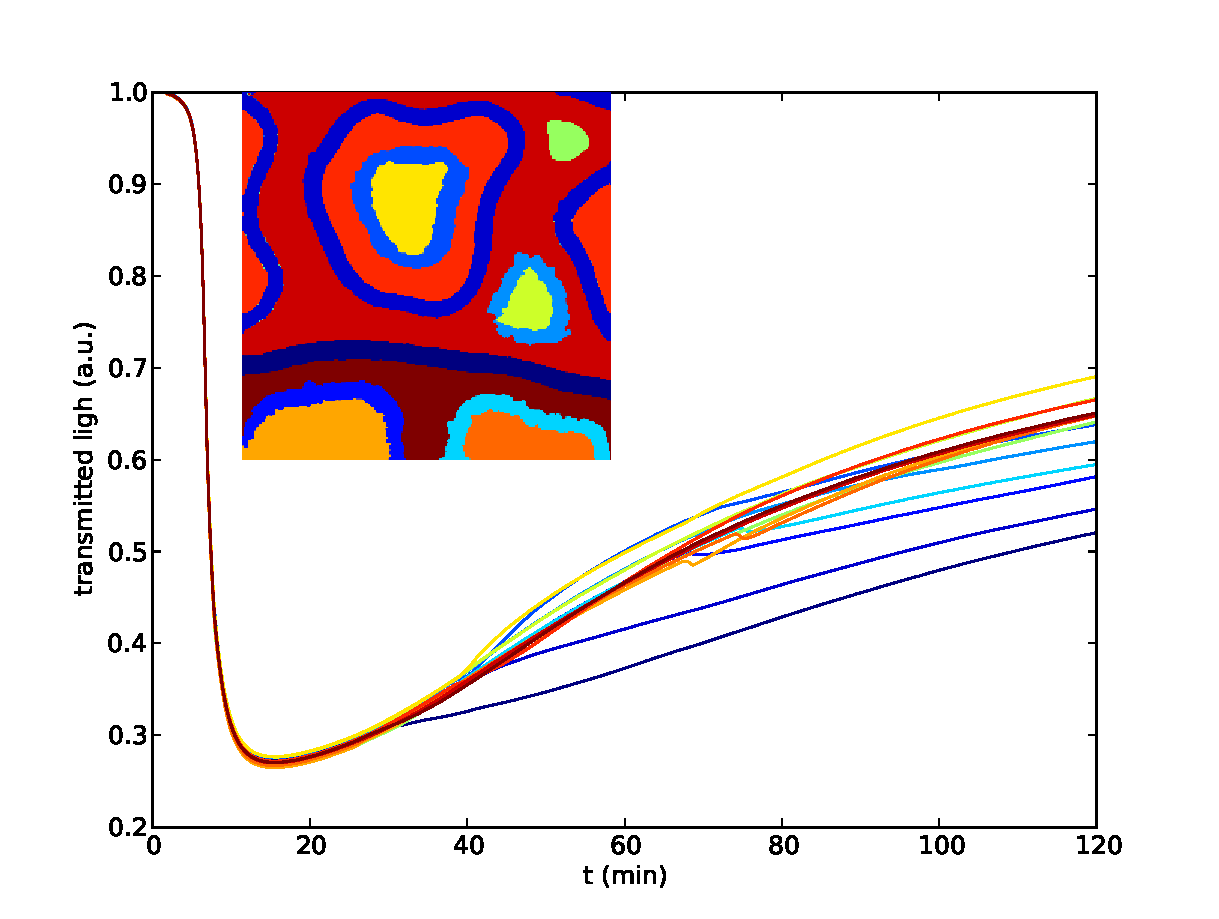
\includegraphics[width=\textwidth]{intensities_by_zones.pdf}
\column{0.4\textwidth}
\begin{itemize}
\item Les zones claires deviennent claires (décollement).
\item Les lignes sombres restent sombres (matière de haut en bas).
\item L'ensemble s’éclaircit.
\end{itemize}
\end{columns}
L'expulsion d'eau est confirmée par confocal après plusieurs semaines (plus qu'une fine couche de gel).
\end{frame}

\begin{frame}{Motifs: Diagramme de phase}
\begin{tikzpicture}
\begin{axis}[%
	name=phasediag,
	xmin=0,xmax=5,xlabel={\% caseinate},
	ymin=0,ymax=5,ylabel={\% GDL},
	legend style={legend pos=north west,}
	]
\addplot[mark=triangle*, green!50!black, only marks,forget plot] coordinates {(4,4) (4,3) (4,2) (4,1)};
\addplot[mark=triangle, green!50!black, only marks] coordinates {(3,3)};
\addplot[mark=square*, red, only marks,forget plot] coordinates {(1,1)};
\addplot[mark=square, red, only marks] coordinates {(2,2)};
\addplot[mark=diamond, orange, only marks] coordinates {(2,1) (3,2) (3,1)};
\legend{Motif, Pas motif, Coexistence};
\addplot[no marks, dotted, black] coordinates {(0,0) (5,5) (10,5) (0,0) (8,2)};
\node at (axis cs:4.5,4.5) {1h};
\node at (axis cs:4.5,1.125) {8h};
\end{axis}
\draw[->] ($(phasediag.north east)+(1em,0)$) -- ($(phasediag.south east)+(1em,0)$) node[midway,right] {$\begin{aligned}
%\tau_\text{prise}&\nearrow\\
G^{\prime}&\nearrow\\
\lambda&\nearrow
\end{aligned}$};
\draw[->] ($(phasediag.north west)+(0,1em)$) -- ($(phasediag.north east)+(0,1em)$) node[midway,above] {$G^{\prime}\nearrow$};
\end{tikzpicture}
\end{frame}

\begin{frame}{Motifs et fractures : longueurs d'onde}
Dans les compositions où on a une loi de puissance à bas $\sigma$ (et donc des fractures) on observe des motifs. Inversement, si la loi est exponentielle (pas de fracture), on n'observe pas de motifs. Est-ce que les motifs sont les fractures à $\sigma=0$ ?

Est-ce que $\lambda_f$ et $\lambda_m$ évoluent de la même façon en fonction des paramètres de contrôles : gap, courbure, composition du gel, G', temps de prise, etc. ?
\end{frame}
\end{document}